% ============================================================
%  Курсова робота
%  Козаріз Володимир
%  Тема: Використання алгоритму Mask R-CNN для розпізнавання
%        об'єктів в системах аероспостереження
%  Львівський національний університет імені Івана Франка
%  Спеціальність F3 Комп'ютерні науки
%  2026
%
%  Компілятор: XeLaTeX (запустити двічі)
%  Шрифт: Times New Roman
% ============================================================

\documentclass[14pt,a4paper]{extreport}

%% ─── Шрифти та мова ─────────────────────────────────────────────────────────
\usepackage{fontspec}
\setmainfont[
  Ligatures = TeX,
  BoldFont  = {Times New Roman Bold},
  ItalicFont= {Times New Roman Italic},
  BoldItalicFont = {Times New Roman Bold Italic}
]{Times New Roman}
\setmonofont[Scale=0.85]{Liberation Mono}

\usepackage{polyglossia}
\setmainlanguage{ukrainian}
\setotherlanguage{english}

%% ─── Поля сторінки ──────────────────────────────────────────────────────────
\usepackage[top=20mm, bottom=20mm, left=30mm, right=10mm,
            headheight=17pt]{geometry}

%% ─── Міжрядковий інтервал та абзацний відступ ───────────────────────────────
\usepackage{setspace}
\onehalfspacing
\setlength{\parindent}{1.25cm}
\setlength{\parskip}{0pt}

%% ─── Нумерація сторінок: арабські цифри, правий верхній кут ─────────────────
\usepackage{fancyhdr}
\pagestyle{fancy}
\fancyhf{}
\fancyhead[R]{\thepage}
\renewcommand{\headrulewidth}{0pt}
\fancypagestyle{plain}{%
  \fancyhf{}%
  \fancyhead[R]{\thepage}%
  \renewcommand{\headrulewidth}{0pt}%
}

%% ─── Заголовки розділів та підрозділів ──────────────────────────────────────
\usepackage{titlesec}

% Розділ: по центру, жирний, БЕЗ крапки
\titleformat{\chapter}[block]
  {\normalfont\bfseries\centering}
  {\thechapter\quad}
  {0pt}
  {}
\titlespacing*{\chapter}{0pt}{0pt}{14pt}

% Підрозділ: з абзацного відступу, звичайний (не жирний), без крапки
\titleformat{\section}[block]
  {\normalfont}
  {\thesection\quad}
  {0pt}
  {}
\titlespacing*{\section}{\parindent}{12pt}{6pt}

% Пункт
\titleformat{\subsection}[block]
  {\normalfont}
  {\thesubsection\quad}
  {0pt}
  {}
\titlespacing*{\subsection}{\parindent}{10pt}{4pt}

%% ─── Нумерація рисунків, таблиць, формул у межах розділу ───────────────────
\usepackage{chngcntr}
\counterwithin{figure}{chapter}
\counterwithin{table}{chapter}
\counterwithin{equation}{chapter}

%% ─── Підписи до рисунків і таблиць ─────────────────────────────────────────
\usepackage{caption}
\DeclareCaptionLabelSeparator{endash}{\space--\space}
\captionsetup[figure]{
  name        = Рисунок,
  labelsep    = endash,
  justification = centering,
  font        = normalsize,
  labelfont   = normalfont,
  position    = below
}
\captionsetup[table]{
  name        = Таблиця,
  labelsep    = endash,
  justification = raggedright,
  singlelinecheck = false,
  font        = normalsize,
  labelfont   = normalfont,
  position    = above
}

%% ─── Таблиці ────────────────────────────────────────────────────────────────
\usepackage{booktabs}
\usepackage{longtable}
\usepackage{array}
\usepackage{multirow}
\usepackage{tabularx}

%% ─── Математика ─────────────────────────────────────────────────────────────
\usepackage{amsmath}
\usepackage{amssymb}

%% ─── Зображення ─────────────────────────────────────────────────────────────
\usepackage{graphicx}
\graphicspath{{figures/}}
\usepackage{float}

%% ─── Лістинги коду ──────────────────────────────────────────────────────────
\usepackage{listings}
\usepackage{xcolor}
\lstset{
  basicstyle    = \small\ttfamily,
  breaklines    = true,
  columns       = fullflexible,
  keepspaces    = true,
  showstringspaces = false,
  frame         = single,
  framesep      = 4pt,
  xleftmargin   = \parindent,
  numbers       = left,
  numberstyle   = \tiny\color{gray},
  stepnumber    = 5,
  tabsize       = 4,
  keywordstyle  = \bfseries,
  commentstyle  = \itshape\color{gray!70},
  stringstyle   = \color{gray!50!black},
}

%% ─── Зміст ──────────────────────────────────────────────────────────────────
\usepackage{tocloft}
\renewcommand{\cftchapfont}{\normalfont}
\renewcommand{\cftchappagefont}{\normalfont}
\renewcommand{\cftchapdotsep}{\cftdotsep}
\renewcommand{\cftsecfont}{\normalfont}
\renewcommand{\cftsecpagefont}{\normalfont}
\setlength{\cftbeforechapskip}{0pt}
\setlength{\cftbeforesecskip}{0pt}
\setlength{\cftbeforetoctitleskip}{0pt}
\setlength{\cftaftertoctitleskip}{10pt}

%% ─── Мікротипографія та переноси URL ────────────────────────────────────────
\PassOptionsToPackage{hyphens}{url}
\usepackage[protrusion=true]{microtype}
\setlength\emergencystretch{6em}

%% ─── Гіперпосилання (без кольорів) ─────────────────────────────────────────
\usepackage[hidelinks,unicode]{hyperref}

%% ─── Бібліографія: «1.» замість «[1]» у списку + без зайвого \clearpage ──────
\makeatletter
\renewcommand\@biblabel[1]{#1.}
\renewenvironment{thebibliography}[1]{%
  \list{\@biblabel{\@arabic\c@enumiv}}{%
    \settowidth\labelwidth{\@biblabel{#1}}%
    \leftmargin\labelwidth
    \advance\leftmargin\labelsep
    \usecounter{enumiv}%
    \let\p@enumiv\@empty
    \renewcommand\theenumiv{\@arabic\c@enumiv}}%
  \sloppy\clubpenalty4000\widowpenalty4000\sfcode`\.\@m}
  {\def\@noitemerr{\@latex@warning{Empty `thebibliography' environment}}\endlist}
\makeatother

%% ─── Допоміжні команди ──────────────────────────────────────────────────────
% Структурний розділ (ВСТУП, ВИСНОВКИ тощо): по центру, жирний
\newcommand{\structchapter}[1]{%
  \clearpage%
  \phantomsection%
  \begin{center}\bfseries#1\end{center}%
  \addcontentsline{toc}{chapter}{#1}%
  \vspace{14pt}%
}

% Команда для рядка «де» після формули
\newcommand{\where}{\par\noindent де\quad}

% Додаток (Додаток А, Б, В …)
\newcounter{appendixno}
\setcounter{appendixno}{0}
\newcommand{\appendixchapter}[2]{%   #1=лitera, #2=title
  \clearpage%
  \phantomsection%
  \begin{center}Додаток~#1\end{center}%
  \begin{center}\bfseries#2\end{center}%
  \addcontentsline{toc}{chapter}{Додаток~#1. #2}%
  \vspace{10pt}%
}

% ─────────────────────────────────────────────────────────────────────────────
\begin{document}
\pagenumbering{arabic}
\setcounter{page}{1}

% ═══════════════════════════════════════════════════════════════════════════
%  ТИТУЛЬНА СТОРІНКА
% ═══════════════════════════════════════════════════════════════════════════
\begin{titlepage}
\thispagestyle{empty}
\begin{center}
\textbf{МІНІСТЕРСТВО ОСВІТИ І НАУКИ УКРАЇНИ}\\[4pt]
\textbf{ЛЬВІВСЬКИЙ НАЦІОНАЛЬНИЙ УНІВЕРСИТЕТ ІМЕНІ ІВАНА ФРАНКА}\\[4pt]
Факультет електроніки та комп'ютерних технологій\\[4pt]
Кафедра програмування
\end{center}

\vspace{10mm}
\begin{center}
\textbf{ВИКОРИСТАННЯ АЛГОРИТМУ MASK R-CNN\\
ДЛЯ РОЗПІЗНАВАННЯ ОБ'ЄКТІВ\\
В СИСТЕМАХ АЕРОСПОСТЕРЕЖЕННЯ}\\[6pt]
Курсова робота\\
за спеціальністю F3 Комп'ютерні науки
\end{center}

\vspace{6mm}
\noindent
\begin{tabular}{@{}p{0.50\textwidth}p{0.45\textwidth}@{}}
 & Виконав: студент \underline{\hspace{1.5cm}} групи \\[4pt]
 & \textbf{Козаріз Володимир} \\[4pt]
 & \underline{\hspace{5.5cm}} \\[2pt]
 & \hspace{1.5cm}\textit{(підпис)} \\[12pt]
 & Науковий керівник: доц. Корчак Ю.~М. \\[4pt]
 & \underline{\hspace{5.5cm}} \\[2pt]
 & \hspace{1.5cm}\textit{(підпис)} \\
\end{tabular}

\vfill
\begin{center}
Львів\,--\,2026
\end{center}
\end{titlepage}

% ═══════════════════════════════════════════════════════════════════════════
%  АНОТАЦІЯ
% ═══════════════════════════════════════════════════════════════════════════
\thispagestyle{empty}
\begin{center}\bfseries АНОТАЦІЯ\end{center}

\noindent Козаріз~В. Використання алгоритму Mask~R-CNN для розпізнавання
об'єктів в системах аероспостереження. Курсова робота за спеціальністю
F3~«Комп'ютерні науки». Львівський національний
університет імені Івана Франка. Львів, 2026.

Досліджено Mask~R-CNN для виявлення військових об'єктів у відеопотоці
БПЛА. Сформовано датасет трьох класів~(солдат, БТР, танк) з відкритих
джерел та псевдо-розмічення відео. Проведено двоетапне навчання в
Detectron2: v1~--- 30\,000~ітерацій на вихідному датасеті;
v2~--- 10\,000~ітерацій на розширеному датасеті. Модель~v2 досягає
mAP@50~=~64,5\% (bbox) та 64,9\% (segm) при 25~FPS на GPU
RTX~4070~Ti~Super. Найбільший приріст від другого етапу:
БТР~(+10,5\%) та солдат~(+5,3\%).

\textbf{Ключові слова:} Mask~R-CNN, БПЛА, сегментація екземплярів,
псевдо-розмічення, Detectron2.

\vspace{6mm}
\begin{center}\bfseries ABSTRACT\end{center}

\noindent Kozariz~V. Application of the Mask~R-CNN Algorithm for Object
Recognition in Aerial Surveillance Systems. Course work, specialty F3
Computer Science. Ivan Franko National University of Lviv.
Lviv, 2026.

The work investigates Mask~R-CNN for military object detection in
UAV-based aerial surveillance. A dataset of three classes~--- soldier,
APC, and tank~--- was assembled from open sources and video
pseudo-labeling. Two-stage training was performed using Detectron2:
v1~--- 30,000~iterations on the initial dataset;
v2~--- 10,000~iterations on the expanded dataset. Model~v2 achieves
mAP@50~=~64.5\% (bbox) and 64.9\% (segm) at 25~FPS on an
RTX~4070~Ti~Super GPU. Largest gains from stage~2:
APC~(+10.5\%) and soldier~(+5.3\%).

\textbf{Keywords:} Mask~R-CNN, UAV, instance segmentation,
pseudo-labeling, Detectron2.

\clearpage

% ═══════════════════════════════════════════════════════════════════════════
%  ЗМІСТ
% ═══════════════════════════════════════════════════════════════════════════
\thispagestyle{empty}
\renewcommand{\contentsname}{\centerline{ЗМІСТ}}
\begin{singlespace}
\tableofcontents
\end{singlespace}
\clearpage

% ═══════════════════════════════════════════════════════════════════════════
%  ПЕРЕЛІК УМОВНИХ ПОЗНАЧЕНЬ
% ═══════════════════════════════════════════════════════════════════════════
\structchapter{ПЕРЕЛІК УМОВНИХ ПОЗНАЧЕНЬ, СИМВОЛІВ, СКОРОЧЕНЬ І ТЕРМІНІВ}

\noindent
\begin{tabular}{@{}p{0.22\textwidth}p{0.72\textwidth}@{}}
AP    & Average Precision~--- середня точність \\
AP@50 & AP при порозі IoU $\geq$~0{,}50 \\
AR    & Average Recall~--- середня повнота \\
БТР   & Бронетранспортер \\
БПЛА  & Безпілотний літальний апарат \\
COCO  & Common Objects in Context~--- стандартний бенчмарк детекції \\
CNN   & Convolutional Neural Network~--- згорткова нейронна мережа \\
FPN   & Feature Pyramid Network~--- мережа пірамідальних ознак \\
FPS   & Frames Per Second~--- кадрів на секунду \\
GPU   & Graphics Processing Unit~--- графічний процесор \\
IoU   & Intersection over Union~--- перетин до об'єднання \\
mAP   & mean Average Precision~--- середнє AP по класах \\
NMS   & Non-Maximum Suppression~--- придушення немаксимумів \\
R-CNN & Region-based CNN~--- регіон-орієнтована CNN \\
RoI   & Region of Interest~--- область інтересу \\
RPN   & Region Proposal Network~--- мережа пропозицій регіонів \\
UAV   & Unmanned Aerial Vehicle~--- безпілотний літальний апарат \\
VRAM  & Video Random Access Memory~--- відеопам'ять \\
\end{tabular}

% ═══════════════════════════════════════════════════════════════════════════
%  ВСТУП
% ═══════════════════════════════════════════════════════════════════════════
\structchapter{ВСТУП}

Розвиток технологій безпілотних літальних апаратів~(БПЛА) суттєво
розширює можливості систем аероспостереження. Автоматизоване виявлення
та ідентифікація наземних об'єктів у відеопотоці БПЛА є актуальною
задачею: специфічні умови аерозйомки~--- нестабільний ракурс, мінливий
масштаб, дрібні об'єкти, камуфляж~--- ускладнюють застосування
стандартних алгоритмів~\cite{liuUAVYOLO2020}.

\textbf{Мета роботи}~--- розробка та дослідження системи виявлення і
розпізнавання об'єктів у відеопотоці з БПЛА на основі Mask~R-CNN,
що забезпечує локалізацію (bounding box) та попіксельну сегментацію.

\textbf{Об'єкт дослідження}~--- автоматичне виявлення та ідентифікація
наземних об'єктів (солдат, БТР, танк) на відеозображеннях із БПЛА.

\textbf{Предмет дослідження}~--- алгоритм Mask~R-CNN, методи його
адаптації до аерофотозображень та реалізація конвеєру від збору даних
до реального інференсу.

\textbf{Методи та апаратура:} двохетапна детекція, transfer learning,
псевдо-розмічення, метрики COCO (mAP, AR). Апаратура: GPU NVIDIA GeForce
RTX~4070~Ti~Super (16~ГБ VRAM).

\textbf{Елементи новизни:} (1)~спеціалізований датасет трьох класів
військових наземних об'єктів; (2)~конвеєр псевдо-розмічення відео з
верифікацією через Roboflow; (3)~двоетапна схема донавчання Mask~R-CNN
із приростом AP@50 для БТР на~$+10{,}5\%$ та солдат на~$+5{,}3\%$.

\textbf{Прогнозні напрямки:} квантизація (INT8) для бортового виконання;
розширення переліку класів; інтеграція GPS-прив'язки для геолокації.

% ═══════════════════════════════════════════════════════════════════════════
%  РОЗДІЛ 1. АНАЛІЗ СТАНУ ПРОБЛЕМНОЇ ГАЛУЗІ
% ═══════════════════════════════════════════════════════════════════════════
\chapter{АНАЛІЗ СТАНУ ПРОБЛЕМНОЇ ГАЛУЗІ}

\section{Задача виявлення об'єктів у системах аероспостереження}

Аероспостереження з використанням БПЛА набуло широкого застосування в
сферах охорони кордонів, моніторингу інфраструктури та ситуаційної
обізнаності. Ключовою складовою таких систем є автоматичне виявлення та
класифікація об'єктів у відеопотоці.

Перспектива зйомки з БПЛА суттєво відрізняється від наземної. До
типових викликів належать~\cite{liuUAVYOLO2020, azimiTracking2020}:

\textbf{Зміна масштабу.} Висота польоту варіюється від 20 до 200~метрів,
через що один і той самий об'єкт може займати від кількох пікселів до
значної частини зображення.

\textbf{Специфічні ракурси.} Камера БПЛА зазвичай спрямована зверху вниз
під кутом від 45° до 90°, тоді як переважна більшість стандартних
датасетів містить об'єкти на рівні очей.

\textbf{Дрібні та щільно розташовані об'єкти.} Солдат з висоти 100~м
займає приблизно $15\times30$ пікселів у зображенні 720p.
Стандартні детектори, оптимізовані під median-розмір об'єктів у
датасеті COCO ($\sim$96~пікселів), погано узагальнюються на такі умови.

\textbf{Камуфляж та зміна вигляду.} Наземна техніка маскується
рослинністю або брезентом; пісковий, лісовий та зимовий камуфляж суттєво
змінює кольорову сигнатуру об'єктів.

\textbf{Динамічний фон.} Рослинність, тіні, різноманітні текстури землі
ускладнюють відокремлення об'єктів від фону.

Для систем підтримки прийняття рішень у реальних умовах
аероспостереження виокремлюються три ключові вимоги: висока точність
(мінімум хибних спрацювань), достатня швидкість (не менше 25~FPS) та
можливість точної локалізації об'єктів. Алгоритми сегментації екземплярів
відповідають усім трьом вимогам, надаючи обмежувальну рамку і попіксельну
маску об'єкта~\cite{maskrcnn2017}.

\section{Огляд сучасних методів детектування та сегментації об'єктів}

Методи виявлення об'єктів поділяються на двохетапні та одноетапні.

\subsection*{Двохетапні детектори}

У цих методах спочатку генерується набір кандидатних областей (region
proposals), а потім кожна класифікується і уточнюється.

\textbf{R-CNN}~\cite{rcnn2014}~--- перший детектор на базі CNN. Витягує
$\sim$2000 пропозицій за допомогою selective search, потім кожну
класифікує окремо. Недолік: $\sim$47~с/зображення.

\textbf{Fast R-CNN}~\cite{fastrcnn2015}~--- обчислює ознаки всього
зображення одноразово; RoI Pooling витягує вектор ознак для кожної
пропозиції. Прискорення в 25~разів порівняно з R-CNN.

\textbf{Faster R-CNN}~\cite{fasterrcnn2017}~--- замінює selective search
мережею регіональних пропозицій (RPN), що використовує спільні ознаки
backbone. Перший детектор, придатний для реального часу ($\sim$5--15~FPS).

\textbf{Mask R-CNN}~\cite{maskrcnn2017}~--- розширює Faster R-CNN гілкою
предсказання бінарних масок. Замінює RoI Pooling на RoI Align для
усунення квантизаційних артефактів.

\subsection*{Одноетапні детектори}

\textbf{YOLO}~\cite{yolo2016} та його наступники (YOLOv5--YOLOv8)~---
безпосередньо передбачають bounding boxes і класи на сітці ознак без
окремого етапу пропозицій. Висока швидкість ($>$100~FPS), але нижча
точність для дрібних об'єктів.

\textbf{SSD}~\cite{ssd2016}~--- мультимасштабне виявлення на кількох
рівнях ознак; гарний компроміс між швидкістю і точністю.

\textbf{DETR}~\cite{detr2020}~--- трансформерна архітектура без ручного
проектування якорів. Конкурентна точність, але тривалий час навчання.

Порівняння ключових характеристик наведено у таблиці~\ref{tab:methods}.

\begin{table}[H]
\caption{Порівняння методів детектування та сегментації об'єктів}
\label{tab:methods}
\centering
\begin{tabularx}{\textwidth}{@{}lXcccc@{}}
\toprule
Метод & Тип & mAP (COCO) & FPS & Сегм. & Рік \\
\midrule
Faster R-CNN & Двохетапний & 37{,}0 & $\sim$15 & Ні & 2015 \\
Mask R-CNN   & Двохетапний & 37{,}1 bbox / 33{,}6 segm & $\sim$12 & Так & 2017 \\
YOLOv7       & Одноетапний & 51{,}4 & $\sim$130 & Ні & 2022 \\
YOLOv8-x     & Одноетапний & 53{,}9 & $\sim$100 & Опц. & 2023 \\
DETR         & Трансф. & 42{,}0 & $\sim$28 & Ні & 2020 \\
\bottomrule
\end{tabularx}
\end{table}

\section{Виклики аерофотозйомки}

Специфіка виявлення об'єктів у аерофото\-зображеннях докладно
досліджувалась у ряді робіт~\cite{liuUAVYOLO2020, azimiTracking2020,
avolaMS2021}.

\textbf{Проблема дрібних об'єктів.} Стандартні архітектури, навчені на
COCO (медіанний розмір об'єкта~---~$\sim$96~пікселів), суттєво знижують
точність при виявленні об'єктів розміром менш ніж 32~пікселі. Feature
Pyramid Network (FPN) частково вирішує цю проблему за рахунок
багаторівневої обробки ознак~\cite{fpn2017}.

\textbf{Доменний зсув.} Датасети загального призначення (COCO,
ImageNet) містять переважно наземні ракурси. Transfer learning
дозволяє ефективно використати навчені ваги як ініціалізацію,
але для досягнення прийнятної точності на аерофотозображеннях
необхідне донавчання на відповідному доменному датасеті~\cite{avolaMS2021}.

\textbf{Клас-дисбаланс.} У аерофотозображеннях одні об'єкти зустрічаються
значно частіше за інші. Перенавчання на частих класах погіршує
узагальнення. Метод псевдо-розмічення дозволяє цілеспрямовано додавати
приклади для рідкісних класів.

\textbf{Перекриття та схожий зовнішній вигляд.} З висоти транспортні
засоби різних типів виглядають схоже за кольором та формою контуру
зверху. Сегментаційна маска дає більше інформації для розрізнення, ніж
bounding box.

\section{Обґрунтування вибору алгоритму Mask R-CNN}

На основі аналізу існуючих методів та вимог задачі можна сформулювати
наступні аргументи на користь Mask~R-CNN:

1. \textbf{Попіксельна сегментація.} Для точної ідентифікації об'єктів
та аналізу їхньої форми важлива маска, а не лише bounding box. Маска
дозволяє розрізняти, наприклад, танк і БТР за контуром корпусу.

2. \textbf{Висока точність.} Двохетапні детектори стабільно перевершують
одноетапні за метрикою AP@50:95 на стандартних бенчмарках.

3. \textbf{Промислова реалізація.} Бібліотека Detectron2 від Meta~AI~---
перевірена у продакшн реалізація Mask~R-CNN з підтримкою навчання з
частковою точністю (AMP/fp16) та стандартною COCO-оцінкою~\cite{detectron2}.

4. \textbf{Transfer learning.} Ваги ResNet-50, попередньо навчені на
COCO~\cite{resnet2016}, містять корисні ознаки форм об'єктів, що суттєво
прискорює донавчання на вузькому доменному датасеті.

5. \textbf{Прийнятна швидкість.} Система аероспостереження з обробкою
на наземній станції допускає затримку 40--50~мс/кадр, яку забезпечує
Mask~R-CNN на сучасному GPU.

% ═══════════════════════════════════════════════════════════════════════════
%  РОЗДІЛ 2. ТЕОРЕТИЧНІ ОСНОВИ MASK R-CNN
% ═══════════════════════════════════════════════════════════════════════════
\chapter{ТЕОРЕТИЧНІ ОСНОВИ MASK R-CNN}

\section{Загальна архітектура Mask R-CNN}

Mask~R-CNN~\cite{maskrcnn2017}~--- двохетапний детектор, що розширює
Faster~R-CNN~\cite{fasterrcnn2017} додатковою гілкою предсказання
бінарних масок. Загальна структура включає чотири основні компоненти:

\begin{itemize}
  \item \textbf{Backbone + FPN}~--- витягує ієрархію просторових ознак з
        вхідного зображення на кількох масштабах.
  \item \textbf{RPN}~--- генерує кандидатні регіони інтересу (RoI).
  \item \textbf{RoI Align}~--- витягує вектор ознак фіксованого розміру
        для кожного RoI без втрат від квантизації.
  \item \textbf{Head}~--- три паралельні підгілки: класифікація об'єкта,
        регресія обмежувальної рамки та сегментаційна маска.
\end{itemize}

Принципова відмінність від Faster~R-CNN полягає в тому, що маскова гілка
навчається \emph{незалежно} від гілки класифікації: на етапі навчання
маска обчислюється лише для класу, передбаченого класифікатором, що
усуває конкуренцію між класами.

\section{Магістральна мережа та Feature Pyramid Network}

Як backbone використовується ResNet-50~\cite{resnet2016}, попередньо
навчений на ImageNet. ResNet-50 складається з чотирьох стадій
$\mathrm{C}_2\ldots\mathrm{C}_5$; кожна наступна стадія зменшує
просторовий розмір карти ознак вдвічі, збільшуючи кількість каналів від
256 до 2048.

Feature Pyramid Network~(FPN)~\cite{fpn2017} вирішує проблему виявлення
об'єктів різних масштабів. FPN будує ієрархію карт ознак у три кроки:

\begin{enumerate}
  \item \textbf{Bottom-up path (знизу вгору):} обчислення ознак
        $\mathrm{C}_2\ldots\mathrm{C}_5$ через ResNet.
  \item \textbf{Top-down path (зверху вниз):} послідовний апсемплінг від
        $\mathrm{C}_5$ до $\mathrm{C}_2$ з кроком 2.
  \item \textbf{Lateral connections (бічні зв'язки):}
        поелементне додавання апсемплінгованої карти до відповідної
        карти bottom-up через $1\!\times\!1$ згортку.
\end{enumerate}

У результаті отримуються карти ознак $\mathrm{P}_2\ldots\mathrm{P}_5$ з
однаковою кількістю каналів~(256), що відповідають різним масштабам:
малі об'єкти виявляються на $\mathrm{P}_2$ (висока просторова роздільна
здатність), великі~--- на $\mathrm{P}_5$.

\section{Мережа регіональних пропозицій}

RPN~--- невелика повнозгорткова мережа, яка ковзає по кожній карті
ознак $\mathrm{P}_l$ і в кожній позиції передбачає:

\begin{itemize}
  \item \textbf{Objectness score}~--- ймовірність того, що якір містить
        об'єкт.
  \item \textbf{Box deltas}~--- поправки для уточнення координат якоря.
\end{itemize}

Функція втрат RPN:

\begin{equation}
  L_{\mathrm{rpn}} = \frac{1}{N_{\mathrm{cls}}}
    \sum_{i} L_{\mathrm{cls}}\!\left(p_i, p^*_i\right)
    + \lambda\,\frac{1}{N_{\mathrm{reg}}}
    \sum_{i} p^*_i\,L_{\mathrm{reg}}\!\left(\mathbf{t}_i,
    \mathbf{t}^*_i\right),
  \label{eq:rpn}
\end{equation}

\where $p_i$~--- передбачена ймовірність об'єкта для якоря~$i$;
$p^*_i$~--- мітка ($1$, якщо IoU~$\geq$~0{,}7);
$\mathbf{t}_i,\mathbf{t}^*_i$~--- передбачений та еталонний вектори
зміщення рамки; $\lambda$~--- балансувальний коефіцієнт.

Після RPN виживають якорі з найвищим objectness score; до них
застосовується Non-Maximum Suppression (NMS) з порогом IoU~=~0{,}7.
Виходом є $\sim$300 RoI-пропозицій для подальшого оброблення.

\section{RoI Align}

RoI Pooling у Fast~R-CNN вносить квантизаційні артефакти через округлення
координат RoI до цілих пікселів. Для задачі сегментації, де маска чутлива
до точного вирівнювання, це критично.

RoI Align~\cite{maskrcnn2017} усуває цю проблему:

\begin{enumerate}
  \item Ділить RoI на рівну сітку комірок (наприклад, $7\!\times\!7$ або
        $14\!\times\!14$).
  \item У кожній комірці рівномірно вибирає 4 вузлові точки (без
        округлення).
  \item Обчислює значення кожної точки як \emph{білінійну інтерполяцію}
        чотирьох найближчих вузлів карти ознак.
  \item Агрегує точки в комірці через max або average pooling.
\end{enumerate}

Білінійна інтерполяція значення $v$ в точці $(x, y)$:

\begin{equation}
  v = \sum_{i,j\in\{0,1\}} w_{ij}\,f\!\left(\lfloor x\rfloor+i,\,
      \lfloor y\rfloor+j\right),
  \label{eq:bilinear}
\end{equation}

\where $w_{ij} = (1-\Delta x + (-1)^i\,\Delta x)(1-\Delta y+(-1)^j\,\Delta y)$~---
білінійні коефіцієнти; $f(p,q)$~--- значення карти ознак у цілому вузлі.

\section{Голови класифікації, регресії та сегментації}

Після RoI Align (вихід $7\!\times\!7$ каналів для bbox, $14\!\times\!14$
для масок) вектор ознак проходить через дві паралельні гілки:

\textbf{Класифікаційна та регресійна гілки.} Два повнозв'язні шари
$(\mathrm{FC}_{1024}\to\mathrm{FC}_{1024})$ з поділом на:
\begin{itemize}
  \item softmax: ймовірності $K\!+\!1$ класів (де $K$~--- кількість
        цільових класів, $+1$~--- фон);
  \item лінійний шар: $4K$ числа для регресії рамки.
\end{itemize}

\textbf{Маскова гілка} (mask head): вхід RoI Align $14\!\times\!14$
проходить через 4~шари $3\!\times\!3$ згорток ($256$ фільтрів) та одну
деконволюцію $2\!\times\!2$ (апсемплінг $\times2$), що дає вихід
$28\!\times\!28$. Виходом є $K$ бінарних карт масок (по одній на клас).

\section{Функції втрат}

Загальна функція втрат Mask~R-CNN:

\begin{equation}
  L = L_{\mathrm{cls}} + L_{\mathrm{box}} + L_{\mathrm{mask}},
  \label{eq:total_loss}
\end{equation}

\where $L_{\mathrm{cls}}$~--- крос-ентропія класифікації;
$L_{\mathrm{box}}$~--- Smooth~L1 для регресії рамки;
$L_{\mathrm{mask}}$~--- середня бінарна крос-ентропія пікселів маски.

\textbf{Smooth L1 (регресія рамки):}

\begin{equation}
  L_{\mathrm{box}} = \sum_{i\in\{x,y,w,h\}}
    \mathrm{smooth}_{L_1}\!\left(t_i - t^*_i\right),
  \quad
  \mathrm{smooth}_{L_1}(x) =
  \begin{cases}
    \dfrac{x^2}{2\beta} & |x| < \beta, \\[4pt]
    |x| - \dfrac{\beta}{2} & |x| \geq \beta,
  \end{cases}
  \label{eq:smooth_l1}
\end{equation}

\where $t_i, t^*_i$~--- передбачений та еталонний параметри рамки;
$\beta = 1$ за замовчуванням.

\textbf{Маскова втрата:}

\begin{equation}
  L_{\mathrm{mask}} = -\frac{1}{m^2}\sum_{1\leq i,j\leq m}
    \left[y_{ij}\log\hat{y}^k_{ij}
    + (1-y_{ij})\log(1-\hat{y}^k_{ij})\right],
  \label{eq:mask_loss}
\end{equation}

\where $y_{ij}$~--- еталонна бінарна маска; $\hat{y}^k_{ij}$~--- передбачена
маска для класу~$k$ (тільки для еталонного класу RoI); $m$~--- розмір
маски ($28\!\times\!28$).

% ═══════════════════════════════════════════════════════════════════════════
%  РОЗДІЛ 3. ПРОГРАМНА РЕАЛІЗАЦІЯ СИСТЕМИ
% ═══════════════════════════════════════════════════════════════════════════
\chapter{ПРОГРАМНА РЕАЛІЗАЦІЯ СИСТЕМИ}

\section{Набір даних}

\subsection*{Класи об'єктів}

Система розроблена для розпізнавання трьох класів наземних об'єктів,
що є типовими цілями в задачах аероспостереження:

\begin{table}[H]
\caption{Класи об'єктів системи розпізнавання}
\label{tab:classes}
\centering
\begin{tabular}{@{}cll@{}}
\toprule
ID & Клас & Опис \\
\midrule
0 & soldier & Солдат (особовий склад) \\
1 & armoured personnel carrier & Бронетранспортер (БТР) \\
2 & tank & Танк \\
\bottomrule
\end{tabular}
\end{table}

\subsection*{Джерела даних}

Набір даних сформовано з трьох джерел:

1. \textbf{Roboflow Universe}~--- відкрита платформа датасетів.
Завантажено набори даних із розміткою військової техніки та особового
складу у форматі COCO~JSON. Для кожного зображення анотації містять
bounding box та полігональну маску~(\texttt{segmentation}).

2. \textbf{iSAID}~\cite{isaid2019}~--- академічний датасет
аерофотозображень (655~451 анотованих екземплярів, 15~категорій).
Використані категорії, що відповідають транспортним засобам та
особовому складу.

3. \textbf{Псевдо-розмічені відеоматеріали}~--- власні відеоматеріали
з відкритих джерел, автоматично анотовані базовою версією моделі
(деталі у підрозділі~3.2).

\subsection*{Обсяг набору даних}

Анотації збережено у форматі COCO~JSON. Кожна анотація містить поля
\texttt{segmentation} (полігон контуру), \texttt{bbox}, \texttt{area},
\texttt{category\_id}, \texttt{iscrowd}.

\begin{table}[H]
\caption{Обсяг набору даних для трьох цільових класів}
\label{tab:dataset}
\centering
\begin{tabular}{@{}lrrrr@{}}
\toprule
Підвибірка & Зображень & Солдат & БТР & Танк \\
\midrule
Навчальна (train) & 1~155 & 668 & 589 & 534 \\
Валідаційна (val) & 302 & 201 & 125 & 125 \\
\textbf{Разом} & \textbf{1~457} & \textbf{869} & \textbf{714} & \textbf{659} \\
\bottomrule
\end{tabular}
\end{table}

Розподіл між підвибірками~--- 80\% / 20\% за зображеннями. Тренувальна
вибірка не перетинається з валідаційною.

\section{Метод псевдо-розмічення}

Метод псевдо-розмічення (pseudo-labeling) дозволяє використати великі
масиви нерозмічених відеоматеріалів для автоматичного отримання
додаткових тренувальних прикладів. Цей підхід особливо ефективний для
класу «солдат», де стандартних датасетів з аерофотозйомки недостатньо.

\textbf{Конвеєр псевдо-розмічення} включає вісім кроків:

\begin{enumerate}
  \item Витяг кадрів із відеофайлів із частотою 1~кадр/с
        (\texttt{pseudo\_label.py}).
  \item Запуск базової моделі Mask~R-CNN з порогом впевненості~0{,}70.
  \item Збереження всіх кадрів, включно з порожніми (нульові детекції
        = негативні приклади).
  \item Конвертація масок у полігони через \texttt{cv2.findContours}.
  \item Експорт у COCO~JSON (\texttt{pseudo\_labels.json}).
  \item Завантаження на платформу Roboflow (\texttt{upload\_roboflow.py}).
  \item Ручна верифікація: перевірка та виправлення автоматичних анотацій.
  \item Злиття перевірених анотацій із основним датасетом
        (\texttt{merge\_\allowbreak datasets.py}).
\end{enumerate}

\begin{table}[H]
\caption{Результати псевдо-розмічення відеоматеріалів}
\label{tab:pseudo}
\centering
\begin{tabular}{@{}lrrrr@{}}
\toprule
Відеофайл & Тривалість & Кадрів витягнуто & З анот. & Порожніх \\
\midrule
yt\_input.mp4  & $\sim$25~хв & 722 & 287 & 435 \\
yt\_input2.mp4 & $\sim$20~хв & 722 & 275 & 447 \\
\textbf{Разом} & $\sim$45~хв & \textbf{1~444} & \textbf{562} & \textbf{882} \\
\bottomrule
\end{tabular}
\end{table}

Кадри без детекцій (882~кадри) збережено як «важкі негативні приклади»
(hard negatives), що допомагає зменшити кількість хибних спрацювань у
фінальній моделі~\cite{liuUAVYOLO2020}.

Ключовий фрагмент логіки збереження кадрів (лістинг~А.3):

\begin{lstlisting}[language=Python, caption={}]
for frame in extracted_frames:
    instances = predictor(frame)["instances"]
    # Зберігаємо кадр незалежно від кількості детекцій
    cv2.imwrite(frame_path, frame)
    if len(instances) == 0:
        continue   # hard negative - без анотацій
    for mask, cls, score in zip(instances.pred_masks,
                                instances.pred_classes,
                                instances.scores):
        segm = mask_to_polygon(mask.numpy())
        coco_annotations.append({
            "category_id": int(cls),
            "segmentation": segm,
            "bbox": mask_to_bbox(mask),
            "score": float(score)
        })
\end{lstlisting}

\section{Навчання моделі}

Навчання проводилось у два послідовні етапи з використанням фреймворку
Detectron2~\cite{detectron2}.

\textbf{Апаратна конфігурація:}
\begin{itemize}
  \item GPU: NVIDIA GeForce RTX~4070~Ti~Super, 16~ГБ VRAM.
  \item CPU: AMD Ryzen (система Nobara Linux).
  \item CUDA 12.4, PyTorch 2.x, Python~3.12.
\end{itemize}

\subsection*{Етап~1 (v1)~--- базове донавчання}

Стартові ваги: \texttt{mask\_rcnn\_R\_50\_FPN\_3x} попередньо навчений на
COCO~\cite{coco2014}. Конфігурація навчання:

\begin{table}[H]
\caption{Гіперпараметри навчання, етап~1 (v1)}
\label{tab:cfg_v1}
\centering
\begin{tabular}{@{}ll@{}}
\toprule
Параметр & Значення \\
\midrule
BASE\_LR & 0{,}001 \\
MAX\_ITER & 30~000 \\
LR steps  & (20~000, 25~000) \\
IMS\_PER\_BATCH & 4 \\
AMP (fp16) & Увімк. \\
ROI\_HEADS.NUM\_CLASSES & 3 \\
\bottomrule
\end{tabular}
\end{table}

За результатами оцінювання на валідаційній вибірці після~v1 модель
досягає AP@50~=~59{,}7\% (bbox) та AP@50~=~60{,}5\% (segm) по трьох
цільових класах. Детальні метрики наведено у розділі~4.

\subsection*{Етап~2 (v2)~--- донавчання на розширеному датасеті}

Стартові ваги ініціалізовані з v1 (\texttt{model\_final.pth}).
Після псевдо-розмічення до тренувального датасету додано 562~нові
анотовані кадри. Знижена базова швидкість навчання запобігає
катастрофічному забуванню при донавчанні:

\begin{table}[H]
\caption{Гіперпараметри навчання, етап~2 (v2)}
\label{tab:cfg_v2}
\centering
\begin{tabular}{@{}ll@{}}
\toprule
Параметр & Значення \\
\midrule
BASE\_LR & 0{,}0005 \\
MAX\_ITER & 10~000 \\
LR steps  & (7~000, 9~000) \\
IMS\_PER\_BATCH & 4 \\
AMP (fp16) & Увімк. \\
\bottomrule
\end{tabular}
\end{table}

Динаміку функції втрат під час навчання~v1 та~v2 наведено у
таблиці~\ref{tab:loss_v2} та на рисунку~\ref{fig:loss_curve}.

\begin{table}[H]
\caption{Динаміка функції втрат під час навчання v2}
\label{tab:loss_v2}
\centering
\begin{tabular}{@{}rrrrr@{}}
\toprule
Ітерація & $L$ (заг.) & $L_{\mathrm{cls}}$ & $L_{\mathrm{mask}}$ & $L_{\mathrm{box}}$ \\
\midrule
1~000 & 0{,}1355 & 0{,}0134 & 0{,}0728 & 0{,}0288 \\
2~000 & 0{,}0994 & 0{,}0129 & 0{,}0624 & 0{,}0239 \\
4~000 & 0{,}1033 & 0{,}0093 & 0{,}0649 & 0{,}0204 \\
6~000 & 0{,}1070 & 0{,}0124 & 0{,}0638 & 0{,}0248 \\
8~000 & 0{,}0971 & 0{,}0090 & 0{,}0598 & 0{,}0241 \\
10~000 & 0{,}1021 & 0{,}0105 & 0{,}0623 & 0{,}0263 \\
\bottomrule
\end{tabular}
\end{table}

\begin{figure}[H]
  \centering
  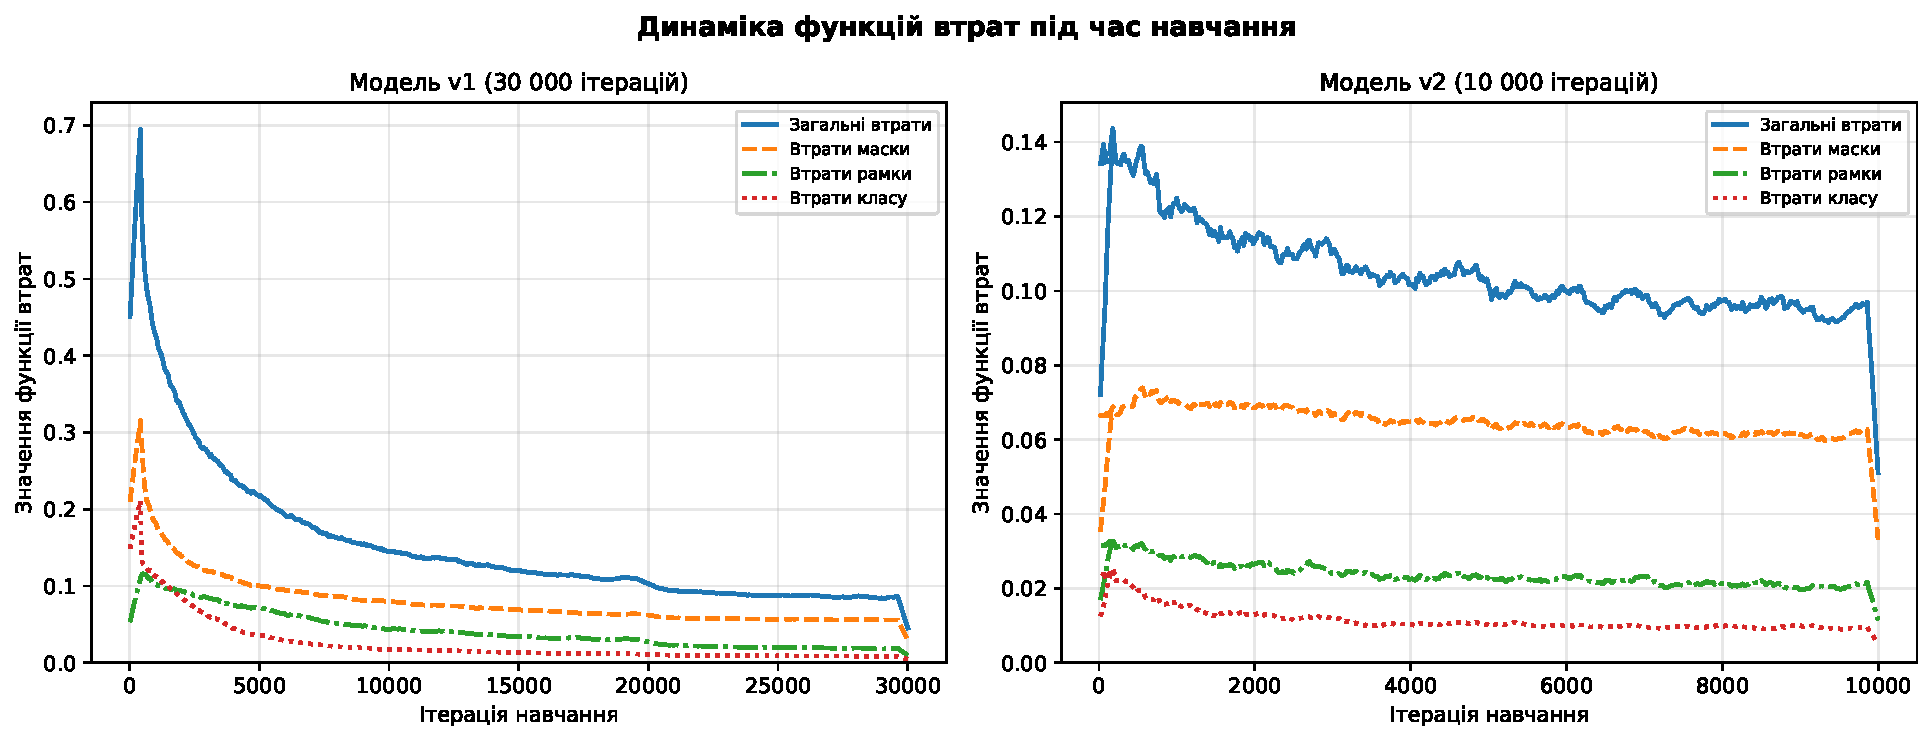
\includegraphics[width=0.88\textwidth]{loss_curve.pdf}
  \caption{Криві функції втрат під час навчання: v1 (30~000 ітерацій, ліворуч) та v2 (10~000 ітерацій, праворуч)}
  \label{fig:loss_curve}
\end{figure}

Втрати стабілізувалися після 2~000--3~000 ітерацій. Це свідчить про
ефективну ініціалізацію з~v1 і відсутність ознак перенавчання.

\section{Конвеєр інференсу та відеообробка}

Для обробки відеопотоку реалізовано скрипт \texttt{mask\_rcnn/infer.py},
що поєднує Mask~R-CNN із CSRT-трекером (OpenCV~4.9).

\textbf{Архітектура системи інференсу:}

\begin{itemize}
  \item Mask~R-CNN запускається з налаштовуваною частотою
        (параметр \texttt{--detect-every}, за замовчуванням кожен кадр).
  \item Для кожного виявленого об'єкта трьох цільових класів
        (солдат, БТР, танк) ініціалізується окремий CSRT-трекер
        (\texttt{cv2.legacy.\allowbreak TrackerCSRT\_create()}).
  \item У проміжних кадрах трекер оновлює позицію без повторного
        запуску нейронної мережі.
  \item Трекер знімається після~1 пропущеної ітерації інференсу без
        відповідного виявлення (\texttt{MAX\_MISSED~=~1}).
  \item Відповідність між новими детекціями та активними трекерами
        визначається за метрикою IoU (мінімальний поріг~0{,}2).
  \item Підтримуються окремі порогові значення впевненості для кожного
        класу (наприклад, \texttt{--thresholds soldier:0.70 apc:0.85}).
\end{itemize}

Кольорове відображення: солдат~--- зелений, БТР~--- помаранчевий,
танк~--- синій; альфа-канал масок~--- 0{,}72.

Система підтримує два режими: збереження результату у відеофайл
(для ретроспективного аналізу) та відображення в реальному часі
(для оперативного моніторингу).

% ═══════════════════════════════════════════════════════════════════════════
%  РОЗДІЛ 4. ТЕСТУВАННЯ
% ═══════════════════════════════════════════════════════════════════════════
\chapter{ТЕСТУВАННЯ}

\section{Методика тестування}

Тестування моделей проводилось на валідаційній підвибірці, яка не
використовувалась під час навчання.

\textbf{Тестова вибірка:} 302~зображення, 451~анотація (201~солдат,
125~БТР, 125~танків).

\textbf{Апаратна платформа:} GPU NVIDIA GeForce RTX~4070~Ti~Super
(16~ГБ VRAM), CUDA~12.4.

\textbf{Протокол оцінювання:} стандартна процедура COCO~\cite{coco2014}.
Для кожного класу обчислюється Average Precision~(AP) за 101 точкою
кривої точність-повнота при IoU від 0{,}5 до 0{,}95 з кроком~0{,}05.
Підсумкові метрики~--- середнє по класах (mean AP).

\textbf{Порівнювані варіанти:}
\begin{itemize}
  \item \textbf{v1}~--- базова модель після початкового донавчання
        (30~000 ітерацій, LR~=~0{,}001).
  \item \textbf{v2}~--- вдосконалена модель після другого етапу
        донавчання на розширеному датасеті (10~000 ітерацій,
        LR~=~0{,}0005).
\end{itemize}

\textbf{Метрики:}

\textit{AP@50 (mAP@50)}~--- середня точність при IoU~$\geq$~0{,}50.
Основна метрика для порівняння.

\textit{AP@75}~--- жорсткіший поріг IoU~$\geq$~0{,}75; характеризує
якість локалізації.

\textit{AR@100}~--- середня повнота при не більше 100 детекцій на
зображення.

Оцінювання проводилось окремо для двох задач: \textbf{bbox}
(локалізація) та \textbf{segm} (сегментація).

\section{Результати базової моделі (v1)}

\begin{table}[H]
\caption{Результати COCO-оцінювання моделі v1}
\label{tab:coco_v1}
\centering
\begin{tabular}{@{}lcccc@{}}
\toprule
 & \multicolumn{2}{c}{Bbox} & \multicolumn{2}{c}{Segm} \\
\cmidrule(lr){2-3}\cmidrule(lr){4-5}
Метрика & v1 & & v1 & \\
\midrule
AP@50   & 0{,}524 & & 0{,}506 & \\
AP@75   & 0{,}340 & & 0{,}346 & \\
AP (small)  & 0{,}118 & & 0{,}151 & \\
AP (medium) & 0{,}327 & & 0{,}368 & \\
AP (large)  & 0{,}410 & & 0{,}424 & \\
AR@100  & 0{,}402 & & 0{,}425 & \\
\bottomrule
\end{tabular}
\end{table}

\begin{table}[H]
\caption{AP@50 за класами, модель v1}
\label{tab:cls_v1}
\centering
\begin{tabular}{@{}lcc@{}}
\toprule
Клас & Bbox AP@50 & Segm AP@50 \\
\midrule
Солдат & 0{,}546 & 0{,}579 \\
БТР    & 0{,}577 & 0{,}580 \\
Танк   & 0{,}668 & 0{,}657 \\
\midrule
\textbf{Середнє} & \textbf{0{,}597} & \textbf{0{,}605} \\
\bottomrule
\end{tabular}
\end{table}

Базова модель v1 показала найвищу точність для класу «танк» (AP@50
bbox~=~66{,}8\%), що пояснюється характерною і добре впізнаваною формою
корпусу. Клас «солдат» є найважчим для виявлення через малий розмір
об'єктів на аерофотозображеннях (AP@50 bbox~=~54{,}6\%).

\section{Результати після розширення датасету (v2)}

\begin{table}[H]
\caption{Результати COCO-оцінювання моделі v2}
\label{tab:coco_v2}
\centering
\begin{tabular}{@{}lcc@{}}
\toprule
Метрика & Bbox & Segm \\
\midrule
AP@50   & 0{,}544 & 0{,}527 \\
AP@75   & 0{,}390 & 0{,}368 \\
AP (small)  & 0{,}113 & 0{,}138 \\
AP (medium) & 0{,}350 & 0{,}381 \\
AP (large)  & 0{,}422 & 0{,}424 \\
AR@100  & 0{,}425 & 0{,}432 \\
\bottomrule
\end{tabular}
\end{table}

\begin{table}[H]
\caption{AP@50 за класами, модель v2}
\label{tab:cls_v2}
\centering
\begin{tabular}{@{}lcc@{}}
\toprule
Клас & Bbox AP@50 & Segm AP@50 \\
\midrule
Солдат & 0{,}599 & 0{,}624 \\
БТР    & 0{,}682 & 0{,}682 \\
Танк   & 0{,}654 & 0{,}642 \\
\midrule
\textbf{Середнє} & \textbf{0{,}645} & \textbf{0{,}649} \\
\bottomrule
\end{tabular}
\end{table}

\section{Порівняльний аналіз v1 та v2}

\begin{table}[H]
\caption{Порівняння AP@50 по класах: v1 vs v2 (bbox)}
\label{tab:compare_bbox}
\centering
\begin{tabular}{@{}lccc@{}}
\toprule
Клас & v1 & v2 & $\Delta$ \\
\midrule
Солдат & 54{,}6\% & 59{,}9\% & \textbf{+5{,}3\%} \\
БТР    & 57{,}7\% & 68{,}2\% & \textbf{+10{,}5\%} \\
Танк   & 66{,}8\% & 65{,}4\% & --1{,}4\% \\
\midrule
\textbf{Середнє} & \textbf{59{,}7\%} & \textbf{64{,}5\%} & \textbf{+4{,}8\%} \\
\bottomrule
\end{tabular}
\end{table}

\begin{table}[H]
\caption{Порівняння AP@50 по класах: v1 vs v2 (segm)}
\label{tab:compare_segm}
\centering
\begin{tabular}{@{}lccc@{}}
\toprule
Клас & v1 & v2 & $\Delta$ \\
\midrule
Солдат & 57{,}9\% & 62{,}4\% & \textbf{+4{,}5\%} \\
БТР    & 58{,}0\% & 68{,}2\% & \textbf{+10{,}2\%} \\
Танк   & 65{,}7\% & 64{,}2\% & --1{,}5\% \\
\midrule
\textbf{Середнє} & \textbf{60{,}5\%} & \textbf{64{,}9\%} & \textbf{+4{,}4\%} \\
\bottomrule
\end{tabular}
\end{table}

Порівняльну діаграму AP@50 за класами наведено на
рисунку~\ref{fig:ap_comparison}.

\begin{figure}[H]
  \centering
  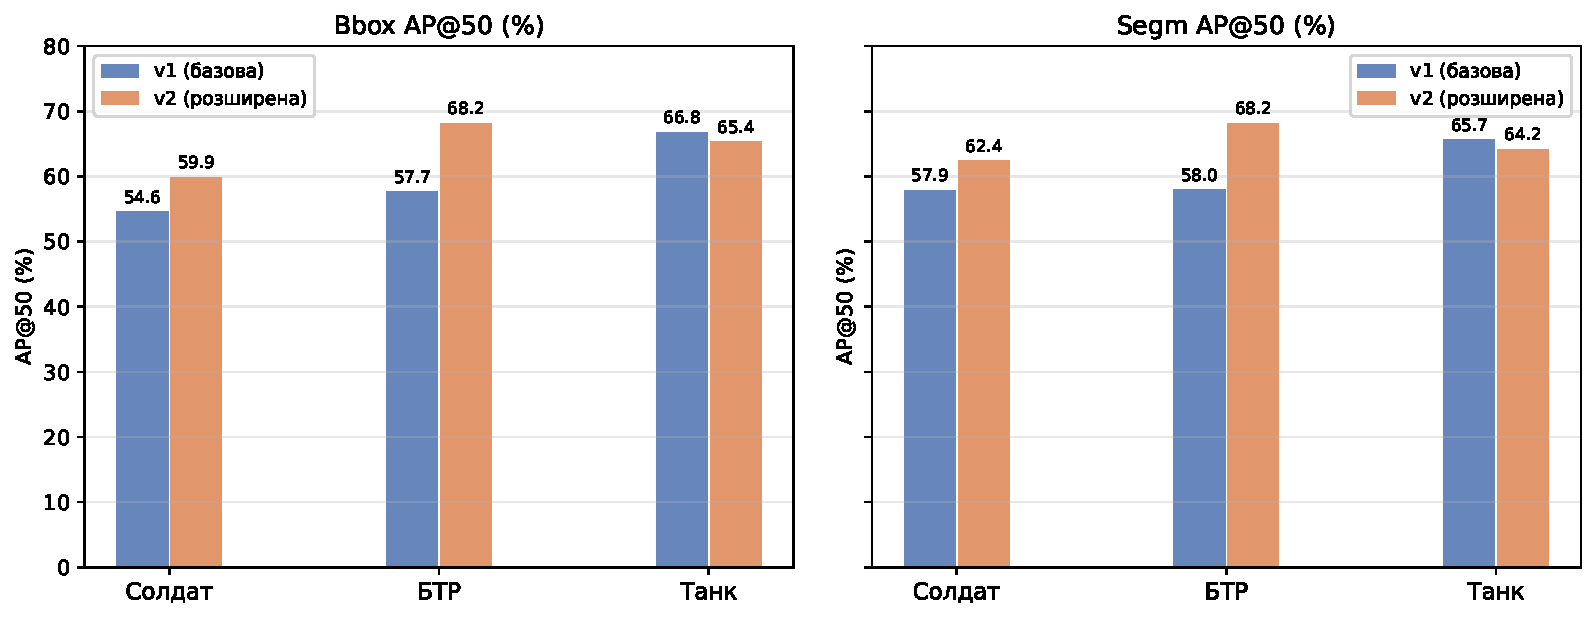
\includegraphics[width=\textwidth]{ap_comparison.pdf}
  \caption{Порівняння AP@50 моделей v1 та v2 за класами та задачами}
  \label{fig:ap_comparison}
\end{figure}

\begin{figure}[H]
  \centering
  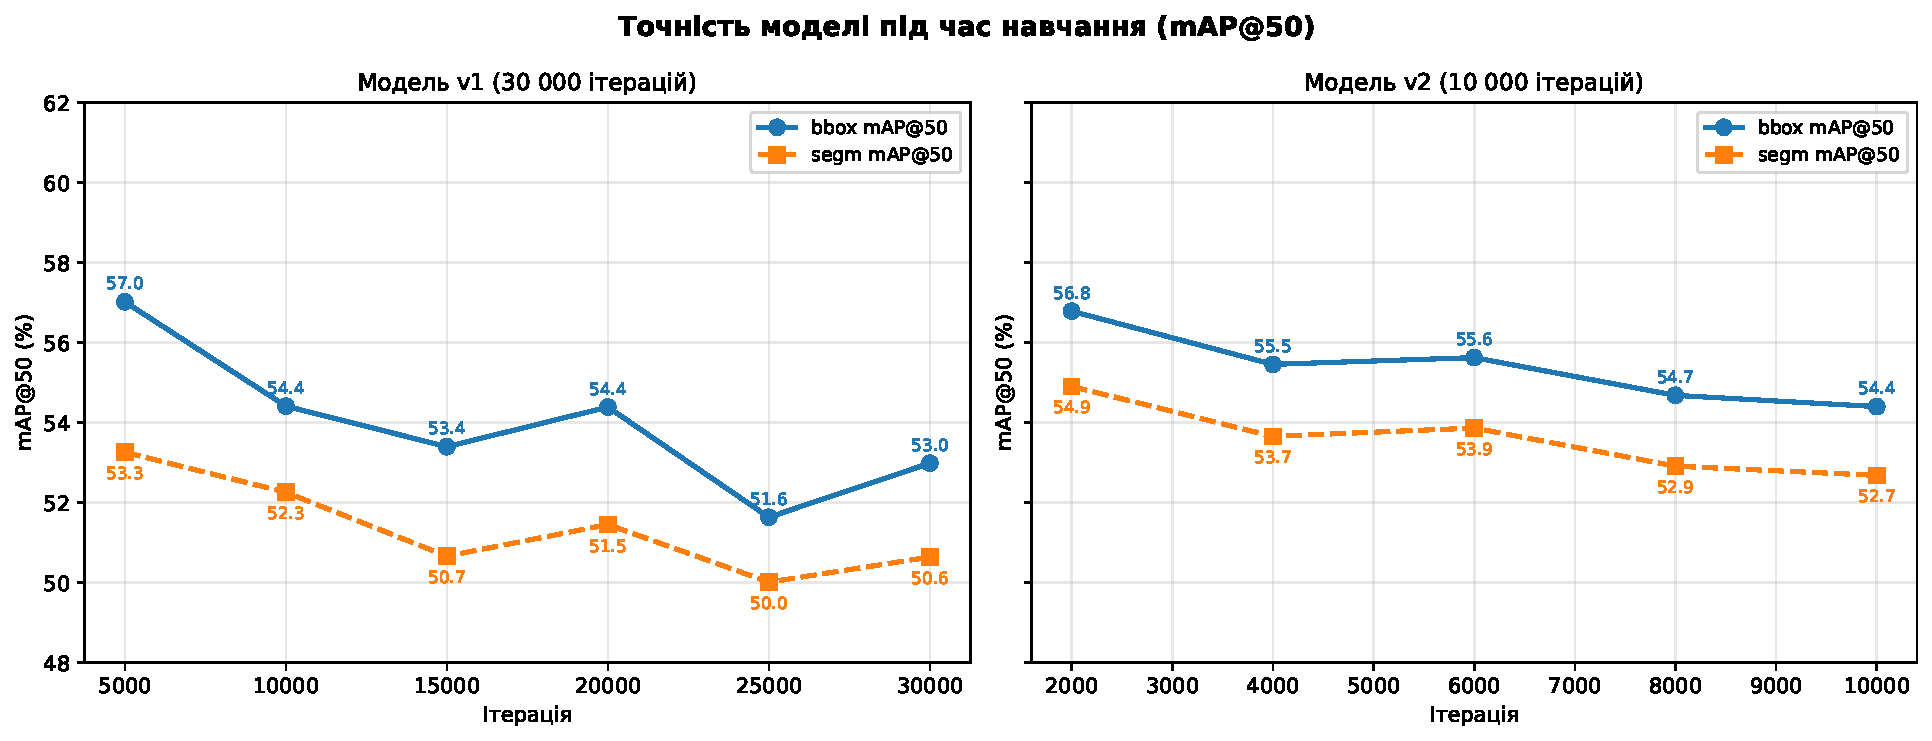
\includegraphics[width=\textwidth]{eval_during_training.pdf}
  \caption{Динаміка mAP@50 на валідаційній вибірці під час навчання:
    v1 (ліворуч, 30~000~ітерацій) та v2 (праворуч, 10~000~ітерацій)}
  \label{fig:eval_during_training}
\end{figure}

\textbf{Аналіз результатів.} Додавання псевдо-розмічених даних дало
найбільший виграш для класів, для яких дані збиралися цілеспрямовано:
\textbf{БТР}~(+10{,}5\% bbox AP@50, +10{,}2\% segm~AP@50) та
\textbf{солдат}~(+5{,}3\% bbox AP@50, +4{,}5\% segm~AP@50). Найбільше
покращення за загальними метриками~--- mAP@75~(+5{,}0\%), що вказує на
підвищення якості локалізації при жорсткому порозі IoU.

Незначне зниження AP для \textbf{танка} на~1{,}4--1{,}5\%~--- типова
ситуація для методу псевдо-розмічення: оскільки відеоматеріали
переважно містили сцени зі знімання на землі, псевдо-розмічені кадри
практично не додали нових прикладів з аерофотозйомки танків, тоді як
розподіл навчальних даних змістився. Балансування датасету може усунути
цей ефект.

\section{Швидкість інференсу}

\begin{table}[H]
\caption{Показники швидкості інференсу (модель v2, GPU RTX~4070~Ti~Super)}
\label{tab:speed}
\centering
\begin{tabular}{@{}lr@{}}
\toprule
Параметр & Значення \\
\midrule
GPU & NVIDIA GeForce RTX~4070~Ti~Super \\
Виміряно кадрів & 295 \\
Середня затримка & 39{,}9~мс \\
Медіанна затримка & 40{,}0~мс \\
СКВ затримки & 0{,}8~мс \\
Мін./Макс. затримка & 37{,}8 / 42{,}6~мс \\
Середнє FPS & 25{,}06 \\
\bottomrule
\end{tabular}
\end{table}

Стабільний час інференсу (СКВ~=~0{,}8~мс) свідчить про рівномірне
навантаження GPU. Значення 25~FPS відповідає вимогам обробки відеопотоку
30~FPS у режимі близькому до реального часу (коефіцієнт використання
0{,}84). Для бортового виконання необхідна подальша оптимізація:
квантизація (INT8) або використання компактнішого backbone
(ResNet-18/34).

\section{Приклади розпізнавання}

На рисунках~\ref{fig:det_soldier_aerial}--\ref{fig:det_apc_road}
наведено приклади роботи моделі v2 на кадрах відеопотоку з БПЛА.
Кольорові маски відображають сегментаційний контур кожного об'єкта;
мітки показують передбачений клас та рівень впевненості.

\begin{figure}[H]
  \centering
  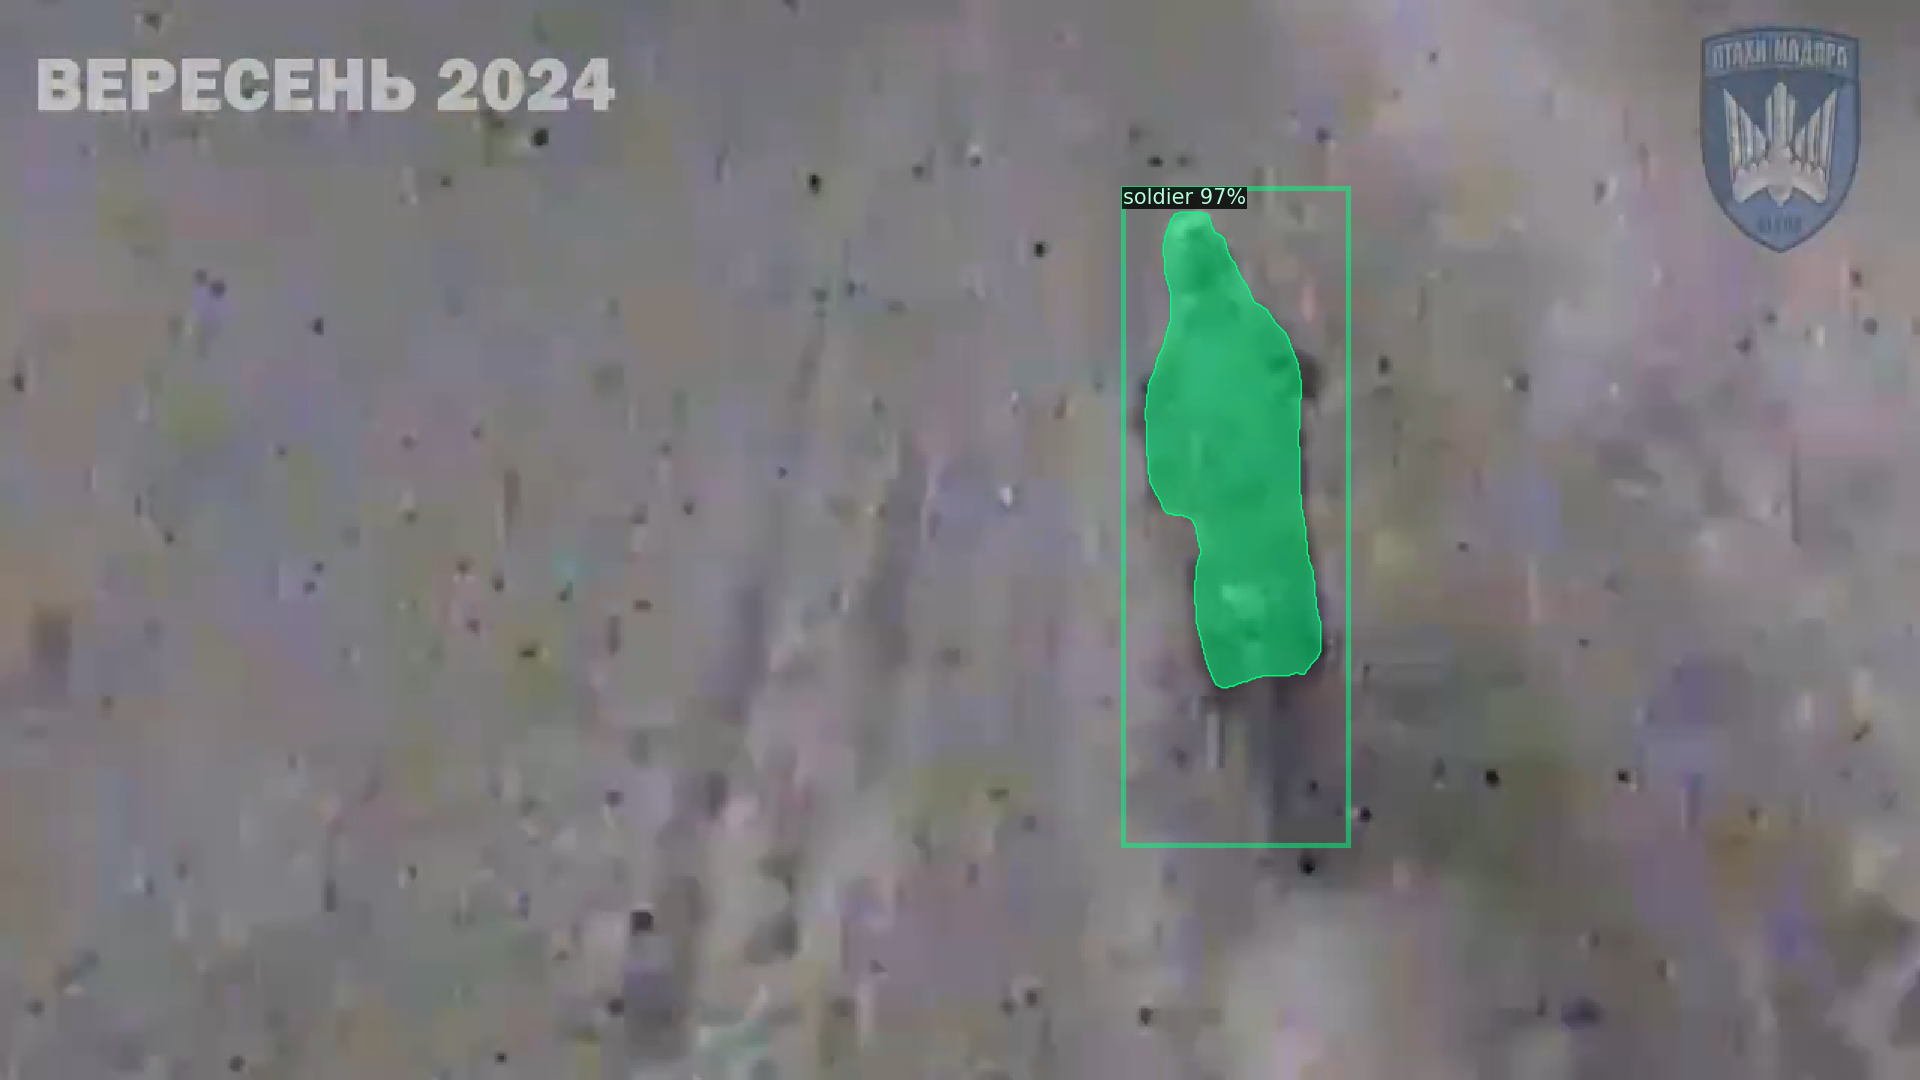
\includegraphics[width=0.82\textwidth]{det_soldier_aerial.jpg}
  \caption{Виявлення солдата: аерофотозйомка згори, впевненість~97\%.
    Одиночний об'єкт класу «солдат» чітко локалізовано на відкритій
    місцевості}
  \label{fig:det_soldier_aerial}
\end{figure}

\begin{figure}[H]
  \centering
  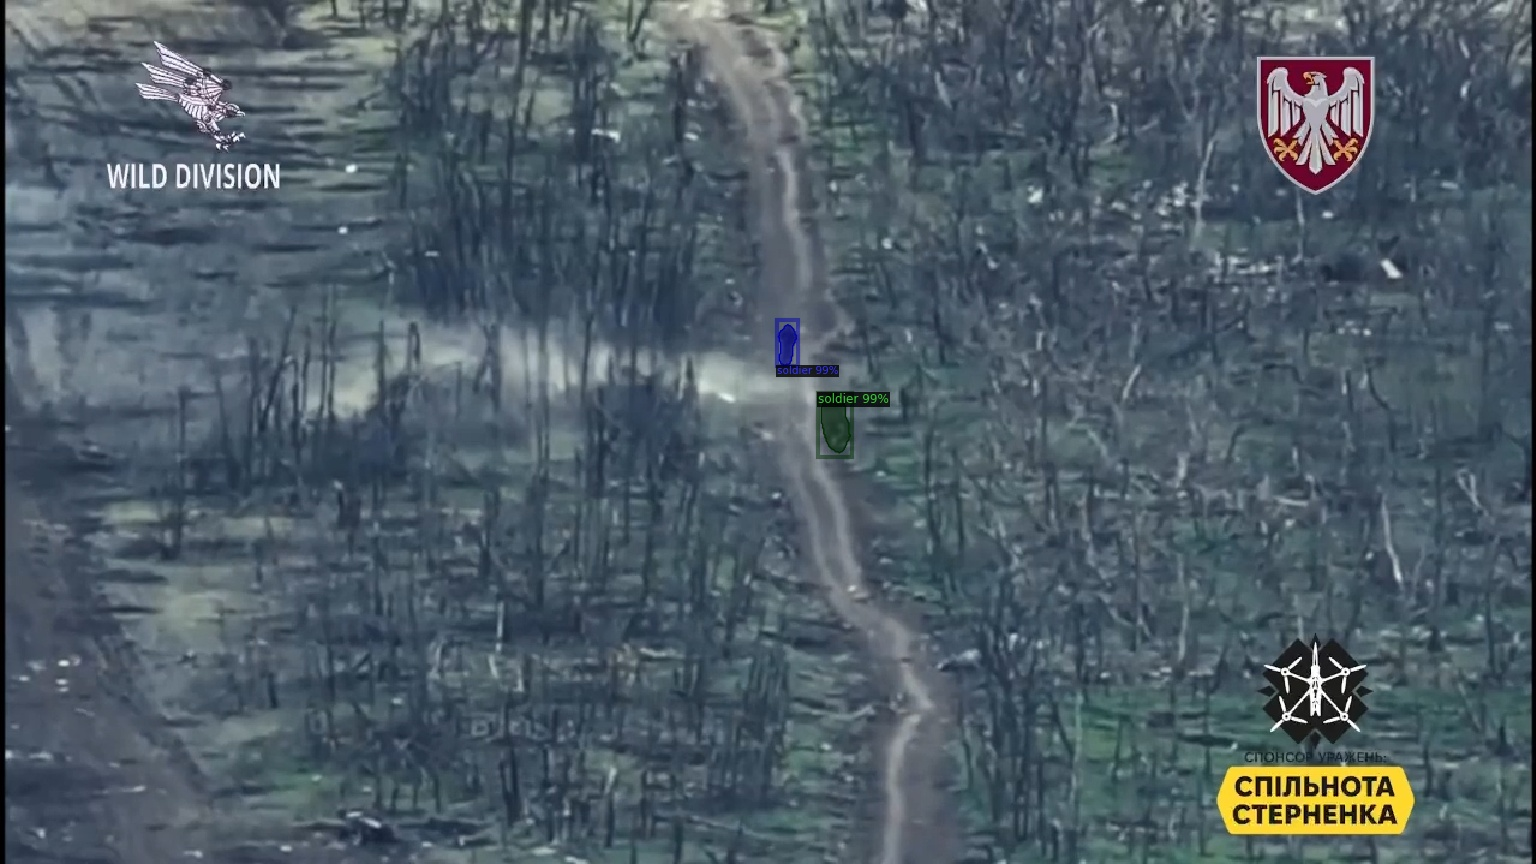
\includegraphics[width=0.82\textwidth]{det_soldiers_multi.jpg}
  \caption{Виявлення двох солдатів у розрідженому лісі.
    Модель розрізняє та сегментує окремих бійців попри часткове
    перекриття рослинністю}
  \label{fig:det_soldiers_multi}
\end{figure}

\begin{figure}[H]
  \centering
  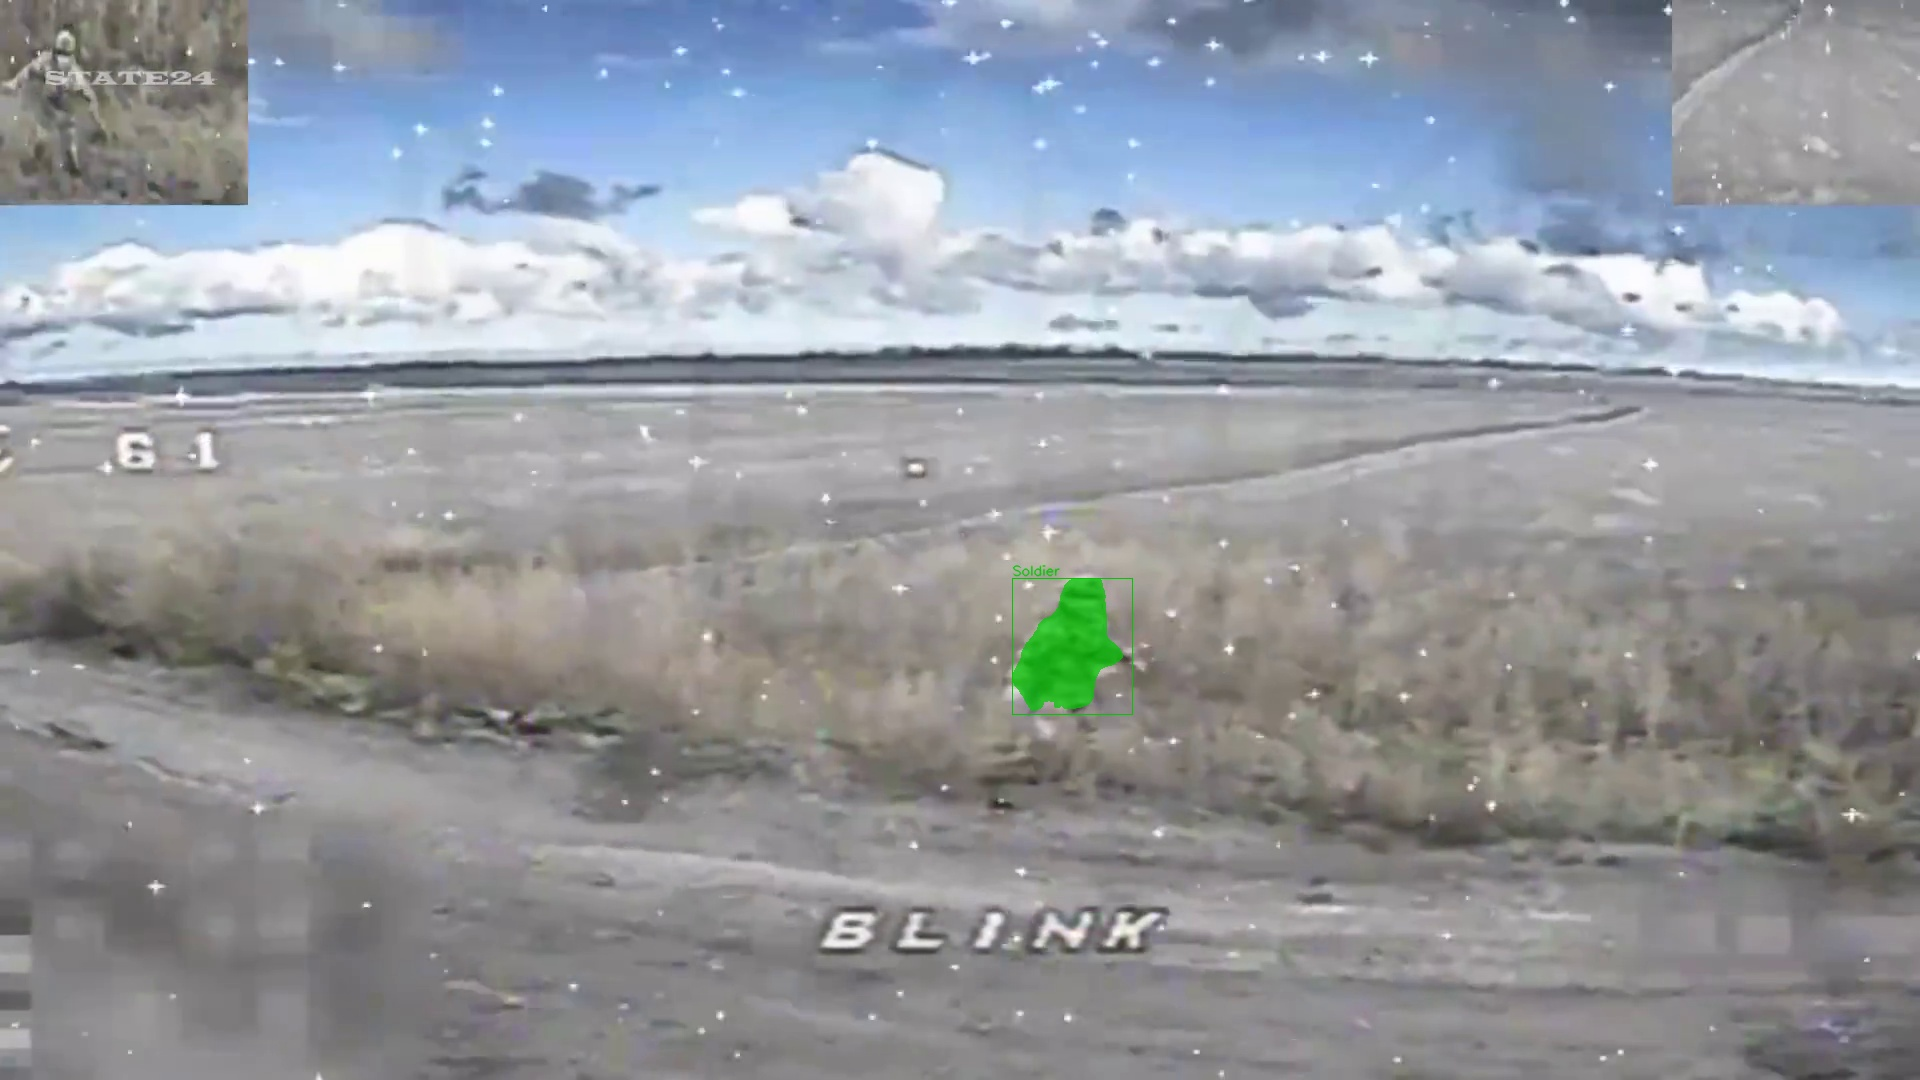
\includegraphics[width=0.82\textwidth]{det_soldier_fpv.jpg}
  \caption{Виявлення солдата у стилі FPV-зйомки.
    Об'єкт розпізнано на відкритій місцевості під нетиповим кутом
    спостереження}
  \label{fig:det_soldier_fpv}
\end{figure}

\begin{figure}[H]
  \centering
  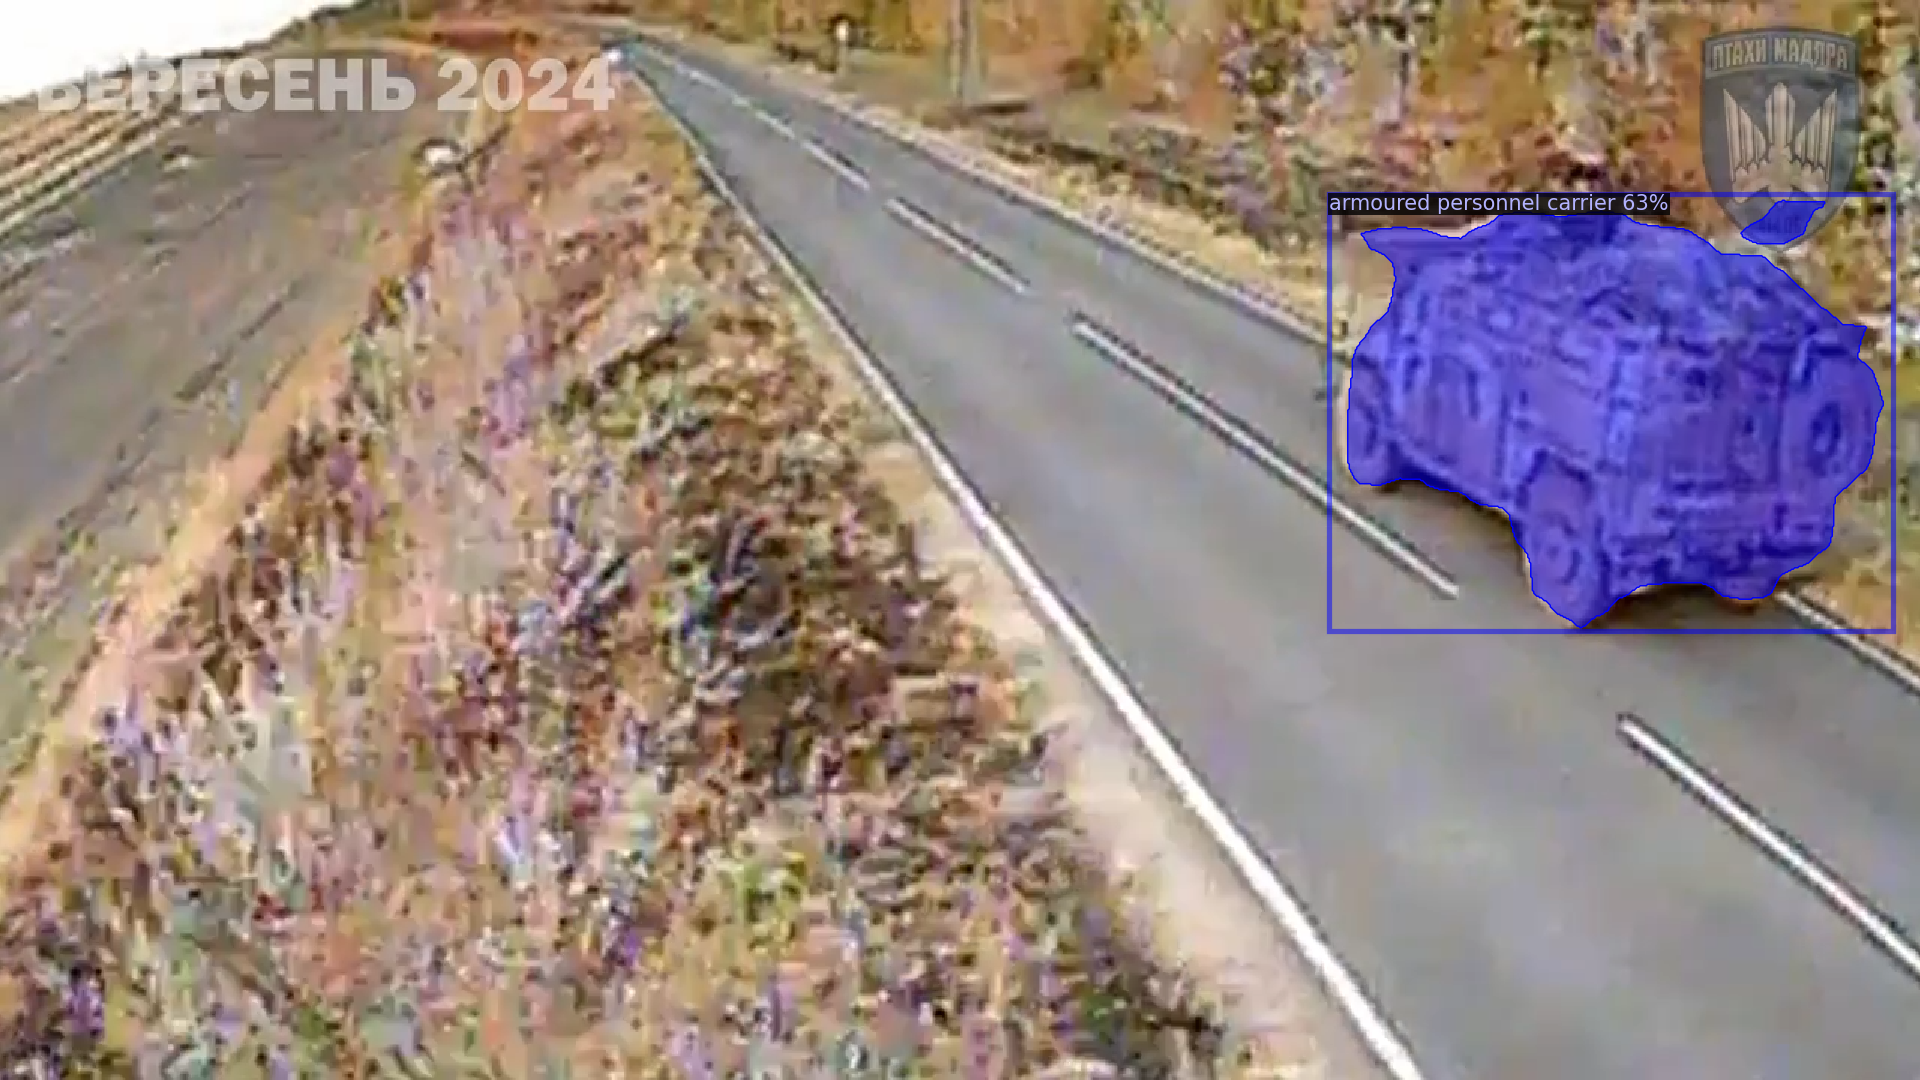
\includegraphics[width=0.82\textwidth]{det_apc_road.jpg}
  \caption{Виявлення бронетранспортера на дорозі, впевненість~63\%.
    Аерофотозйомка; сегментаційна маска обводить корпус БТР}
  \label{fig:det_apc_road}
\end{figure}


% ═══════════════════════════════════════════════════════════════════════════
%  ВИСНОВКИ
% ═══════════════════════════════════════════════════════════════════════════
\structchapter{ВИСНОВКИ}

У курсовій роботі досліджено та реалізовано систему виявлення і
розпізнавання об'єктів у відеопотоці з БПЛА на основі алгоритму
Mask~R-CNN.

У процесі виконання роботи:

--- проведено аналіз сучасних методів комп'ютерного зору для задач
детектування та сегментації об'єктів на аерофотозображеннях; обґрунтовано
вибір Mask~R-CNN як двохетапного детектора, що забезпечує попіксельну
сегментацію при прийнятній швидкості інференсу;

--- детально розглянуто архітектуру Mask~R-CNN: FPN-backbone
(ResNet-50), мережу регіональних пропозицій~(RPN), механізм RoI~Align
та паралельні гілки класифікації, регресії рамки і маски; виведено та
описано функції втрат;

--- сформовано власний набір даних із трьох класів наземних
об'єктів~(солдат, БТР, танк): 1~155~навчальних і 302~валідаційних
зображень, 2~242~анотації; датасет зібрано з публічних аерофотоджерел
та іSAID;

--- розроблено конвеєр псевдо-розмічення відеоматеріалів: витяг
кадрів~(1~кадр/с), автоматичне анотування базовою моделлю, ручна
верифікація на платформі Roboflow та злиття з основним датасетом;
оброблено 1~444~кадри з двох відеофайлів, отримано 562~нових анотованих
кадри;

--- виконано двоетапне навчання: базова модель~v1 (30~000~ітерацій,
LR~=~0{,}001) досягає середнього AP@50~=~59{,}7\% (bbox), 60{,}5\%
(segm); після другого етапу (v2, 10~000~ітерацій на розширеному
датасеті) показники зростають до \textbf{64{,}5\%} (bbox) та
\textbf{64{,}9\%} (segm);

--- показано, що псевдо-розмічення підвищує AP@50 для класу «солдат»
на \textbf{5{,}3\%} та для класу «БТР» на \textbf{10{,}5\%} (bbox);

--- реалізовано конвеєр відеоінференсу з CSRT-трекером; середня затримка
інференсу на GPU NVIDIA RTX~4070~Ti~Super складає \textbf{39{,}9~мс}
(25~FPS).

Практична цінність роботи: розроблена система може бути застосована у
наземних станціях аероспостереження для автоматизованого виявлення та
відстеження солдатів, бронетранспортерів і танків у відеопотоці з БПЛА.

Напрямки подальшого розвитку: оптимізація моделі для бортового
виконання (квантизація INT8, компактний backbone ResNet-18); розширення
переліку класів; дослідження одноетапних методів сегментації (YOLACT,
SAM~2) для підвищення FPS; інтеграція GPS-прив'язки для геолокації
виявлених об'єктів.

% ═══════════════════════════════════════════════════════════════════════════
%  СПИСОК ВИКОРИСТАНИХ ДЖЕРЕЛ
% ═══════════════════════════════════════════════════════════════════════════
\structchapter{СПИСОК ВИКОРИСТАНИХ ДЖЕРЕЛ}

\begin{thebibliography}{15}

\bibitem{liuUAVYOLO2020}
Liu M., Wang X., Zhou A., Fu X., Ma Y., Piao C. UAV-YOLO: Small object
detection on unmanned aerial vehicle perspective. \textit{Sensors}. 2020.
Vol.~20, No.~8. P.~2238.
URL: \url{https://www.mdpi.com/1424-8220/20/8/2238}

\bibitem{azimiTracking2020}
Azimi S.~M., Kraus M., Bahmanyar R., Reinartz P. Multiple pedestrians
and vehicles tracking in aerial imagery: A comprehensive study.
\textit{arXiv}. 2020. arXiv:2010.09689.
URL: \url{https://arxiv.org/abs/2010.09689}

\bibitem{maskrcnn2017}
He K., Gkioxari G., Dollár P., Girshick R. Mask R-CNN.
\textit{Proceedings of the IEEE International Conference on Computer
Vision (ICCV)}, Venice, Italy, 22--29 October 2017. P.~2961--2969.
URL: \url{https://openaccess.thecvf.com/content_iccv_2017/html/He_Mask_R-CNN_ICCV_2017_paper.html}

\bibitem{rcnn2014}
Girshick R., Donahue J., Darrell T., Malik J. Rich feature hierarchies
for accurate object detection and semantic segmentation.
\textit{Proceedings of the IEEE CVPR}, Columbus, OH, 23--28 June 2014.
P.~580--587.
URL: \url{https://openaccess.thecvf.com/content_cvpr_2014/html/Girshick_Rich_Feature_Hierarchies_2014_CVPR_paper.html}

\bibitem{fastrcnn2015}
Girshick R. Fast R-CNN.
\textit{Proceedings of the IEEE ICCV}, Santiago, Chile, 7--13 December
2015. P.~1440--1448.
URL: \url{https://ieeexplore.ieee.org/document/7410526}

\bibitem{fasterrcnn2017}
Ren S., He K., Girshick R., Sun J. Faster R-CNN: Towards real-time
object detection with region proposal networks.
\textit{IEEE Transactions on Pattern Analysis and Machine Intelligence}.
2017. Vol.~39, No.~6. P.~1137--1149.
URL: \url{https://ieeexplore.ieee.org/document/7485869}

\bibitem{yolo2016}
Redmon J., Divvala S., Girshick R., Farhadi A. You only look once:
Unified, real-time object detection.
\textit{Proceedings of the IEEE CVPR}, Las Vegas, NV, 27--30 June 2016.
P.~779--788.
URL: \url{https://www.cv-foundation.org/openaccess/content_cvpr_2016/html/Redmon_You_Only_Look_CVPR_2016_paper.html}

\bibitem{ssd2016}
Liu W., Anguelov D., Erhan D., Szegedy C., Reed S., Fu C.-Y., Berg A.~C.
SSD: Single shot multibox detector.
\textit{Proceedings of the ECCV}, Amsterdam, 11--14 October 2016.
P.~21--37.
URL: \url{https://link.springer.com/chapter/10.1007/978-3-319-46448-0_2}

\bibitem{detr2020}
Carion N., Massa F., Synnaeve G., Usunier N., Kirillov A., Zagoruyko S.
End-to-end object detection with transformers.
\textit{Proceedings of the ECCV}, Glasgow, 23--28 August 2020.
P.~213--229.
URL: \url{https://link.springer.com/chapter/10.1007/978-3-030-58452-8_13}

\bibitem{avolaMS2021}
Avola D., Cinque L., Diko A., Fagioli A., Foresti G.~L., Mecca A.,
Pannone D., Piciarelli C. MS-Faster R-CNN: Multi-stream backbone for
improved Faster R-CNN object detection and aerial tracking from UAV
images. \textit{Remote Sensing}. 2021. Vol.~13, No.~9. P.~1670.
URL: \url{https://www.mdpi.com/2072-4292/13/9/1670}

\bibitem{resnet2016}
He K., Zhang X., Ren S., Sun J. Deep residual learning for image
recognition.
\textit{Proceedings of the IEEE CVPR}, Las Vegas, NV, 27--30 June 2016.
P.~770--778.
URL: \url{https://openaccess.thecvf.com/content_cvpr_2016/html/He_Deep_Residual_Learning_CVPR_2016_paper.html}

\bibitem{fpn2017}
Lin T.-Y., Dollár P., Girshick R., He K., Hariharan B., Belongie S.
Feature pyramid networks for object detection.
\textit{Proceedings of the IEEE CVPR}, Honolulu, HI, 21--26 July 2017.
P.~2117--2125.
URL: \url{https://openaccess.thecvf.com/content_cvpr_2017/html/Lin_Feature_Pyramid_Networks_CVPR_2017_paper.html}

\bibitem{isaid2019}
Waqas Zamir S., Arora A., Gupta A., Khan S., Sun G., Shao L., Xia G.-S.,
Bai X., Yan W., Bhatt J.~S. iSAID: A large-scale dataset for instance
segmentation in aerial images.
\textit{Proceedings of the IEEE/CVF CVPRW}, Long Beach, CA, 16--20 June
2019. P.~28--37.
URL: \url{https://openaccess.thecvf.com/content_CVPRW_2019/html/DOAI/Waqas_Zamir_iSAID_A_Large-scale_Dataset_for_Instance_Segmentation_in_Aerial_Images_CVPRW_2019_paper.html}

\bibitem{coco2014}
Lin T.-Y., Maire M., Belongie S., Hays J., Perona P., Ramanan D.,
Dollár P., Zitnick C.~L. Microsoft COCO: Common objects in context.
\textit{Proceedings of the ECCV}, Zurich, 6--12 September 2014.
P.~740--755.
URL: \url{https://link.springer.com/chapter/10.1007/978-3-319-10602-1_48}

\bibitem{detectron2}
Wu Y., Kirillov A., Massa F., Lo W.-Y., Girshick R. Detectron2.
\textit{Meta AI Research}. 2019.
URL: \url{https://github.com/facebookresearch/detectron2}

\end{thebibliography}

% ═══════════════════════════════════════════════════════════════════════════
%  ДОДАТКИ
% ═══════════════════════════════════════════════════════════════════════════

\appendixchapter{А}{Лістинг коду реєстрації набору даних}

Файл \texttt{mask\_rcnn/dataset.py}~--- реєстрація наборів даних iSAID та
military у форматі COCO для Detectron2.

\begin{lstlisting}[language=Python]
from detectron2.data.datasets import register_coco_instances
from detectron2.data import MetadataCatalog

MILITARY_CLASSES = ["air-fighter", "armoured personnel carrier", "bomber", "soldier", "tank"]


def register_isaid(root: str = "detectron2/datasets/iSAID"):
    register_coco_instances(
        "isaid_train",
        {},
        f"{root}/train/iSAID_train_patches.json",
        f"{root}/train/images",
    )
    register_coco_instances(
        "isaid_val",
        {},
        f"{root}/val/iSAID_val_patches.json",
        f"{root}/val/images",
    )


def register_military(root: str = "detectron2/datasets"):
    register_coco_instances(
        "military_train",
        {},
        f"{root}/military_train.json",
        f"{root}/train",
    )
    register_coco_instances(
        "military_val",
        {},
        f"{root}/military_val.json",
        f"{root}/train",
    )
    MetadataCatalog.get("military_train").thing_classes = MILITARY_CLASSES
    MetadataCatalog.get("military_val").thing_classes = MILITARY_CLASSES
\end{lstlisting}

\appendixchapter{Б}{Лістинг коду навчання моделі}

Файл \texttt{mask\_rcnn/train.py}~--- скрипт навчання на базі
\texttt{DefaultTrainer} з COCO-оцінюванням.

\begin{lstlisting}[language=Python]
import argparse
import os
import sys

from detectron2.config import get_cfg
from detectron2.engine import DefaultTrainer
from detectron2.evaluation import COCOEvaluator

sys.path.insert(0, os.path.dirname(__file__))
from dataset import register_isaid, register_military


class Trainer(DefaultTrainer):
    @classmethod
    def build_evaluator(cls, cfg, dataset_name, output_folder=None):
        if output_folder is None:
            output_folder = os.path.join(cfg.OUTPUT_DIR, "eval")
        return COCOEvaluator(dataset_name, output_dir=output_folder)


def main():
    parser = argparse.ArgumentParser()
    parser.add_argument("--config", required=True)
    parser.add_argument("--resume", action="store_true")
    parser.add_argument("opts", nargs=argparse.REMAINDER)
    args = parser.parse_args()

    register_isaid()
    register_military()

    cfg = get_cfg()
    cfg.merge_from_file(args.config)
    cfg.merge_from_list(args.opts)
    cfg.freeze()

    os.makedirs(cfg.OUTPUT_DIR, exist_ok=True)
    trainer = Trainer(cfg)
    trainer.resume_or_load(resume=args.resume)
    trainer.train()


if __name__ == "__main__":
    main()
\end{lstlisting}

\appendixchapter{В}{Лістинг коду оцінювання моделі}

Файл \texttt{mask\_rcnn/evaluate.py}~--- запуск COCO-оцінювання на
заданому контрольному пункті.

\begin{lstlisting}[language=Python]
import argparse
import os
import sys

from detectron2.config import get_cfg
from detectron2.checkpoint import DetectionCheckpointer
from detectron2.engine import DefaultTrainer
from detectron2.evaluation import COCOEvaluator, inference_on_dataset
from detectron2.data import build_detection_test_loader

sys.path.insert(0, os.path.dirname(__file__))
from dataset import register_isaid, register_military


def main():
    parser = argparse.ArgumentParser()
    parser.add_argument("--config", required=True)
    parser.add_argument("--weights", required=True)
    parser.add_argument("--dataset", required=True)
    args = parser.parse_args()

    register_isaid()
    register_military()

    cfg = get_cfg()
    cfg.merge_from_file(args.config)
    cfg.MODEL.WEIGHTS = args.weights
    cfg.MODEL.ROI_HEADS.SCORE_THRESH_TEST = 0.05
    cfg.freeze()

    model = DefaultTrainer.build_model(cfg)
    DetectionCheckpointer(model).load(cfg.MODEL.WEIGHTS)
    model.eval()
    evaluator = COCOEvaluator(args.dataset,
                              output_dir=os.path.join(cfg.OUTPUT_DIR, "eval"))
    loader = build_detection_test_loader(cfg, args.dataset)
    inference_on_dataset(model, loader, evaluator)


if __name__ == "__main__":
    main()
\end{lstlisting}

\appendixchapter{Г}{Лістинг коду псевдо-розмічення}

Файл \texttt{mask\_rcnn/pseudo\_label.py}~--- витяг кадрів з відео,
автоматичне анотування Mask~R-CNN та збереження COCO~JSON.

\begin{lstlisting}[language=Python]
import argparse
import json
import os
import sys
import cv2
import numpy as np

from detectron2.config import get_cfg
from detectron2.engine import DefaultPredictor

sys.path.insert(0, os.path.dirname(__file__))
from dataset import register_isaid, register_military, MILITARY_CLASSES


def mask_to_polygon(binary_mask):
    contours, _ = cv2.findContours(
        binary_mask.astype(np.uint8),
        cv2.RETR_EXTERNAL,
        cv2.CHAIN_APPROX_SIMPLE,
    )
    polygons = []
    for c in contours:
        if cv2.contourArea(c) < 4:
            continue
        poly = c.flatten().tolist()
        if len(poly) >= 6:
            polygons.append(poly)
    return polygons


def build_predictor(config, weights, threshold):
    register_isaid()
    register_military()
    cfg = get_cfg()
    cfg.merge_from_file(config)
    cfg.MODEL.WEIGHTS = weights
    cfg.MODEL.ROI_HEADS.SCORE_THRESH_TEST = threshold
    cfg.freeze()
    return DefaultPredictor(cfg)


def process_videos(videos, out_dir, sample_fps, threshold, config, weights):
    images_dir = os.path.join(out_dir, "images")
    os.makedirs(images_dir, exist_ok=True)
    predictor = build_predictor(config, weights, threshold)
    coco = {
        "info": {"description": "Pseudo-labeled military dataset"},
        "categories": [
            {"id": i + 1, "name": name, "supercategory": "military"}
            for i, name in enumerate(MILITARY_CLASSES)
        ],
        "images": [],
        "annotations": [],
    }
    img_id = 1
    ann_id = 1
    for video_path in videos:
        cap = cv2.VideoCapture(video_path)
        native_fps = cap.get(cv2.CAP_PROP_FPS) or 30
        total_frames = int(cap.get(cv2.CAP_PROP_FRAME_COUNT))
        step = max(1, int(round(native_fps / sample_fps)))
        video_name = os.path.splitext(os.path.basename(video_path))[0]
        frame_idx = 0
        saved = 0
        annotated = 0
        while True:
            ret, frame = cap.read()
            if not ret:
                break
            if frame_idx % step == 0:
                instances = predictor(frame)["instances"].to("cpu")
                H, W = frame.shape[:2]
                fname = f"{video_name}_f{frame_idx:07d}.jpg"
                fpath = os.path.join(images_dir, fname)
                cv2.imwrite(fpath, frame, [cv2.IMWRITE_JPEG_QUALITY, 95])
                coco["images"].append({
                    "id": img_id, "file_name": fname,
                    "width": W, "height": H,
                })
                if len(instances) > 0:
                    boxes = instances.pred_boxes.tensor.tolist()
                    classes = instances.pred_classes.tolist()
                    scores = instances.scores.tolist()
                    masks = (instances.pred_masks.numpy()
                             if instances.has("pred_masks") else None)
                    for i, (box, cls, score) in enumerate(
                            zip(boxes, classes, scores)):
                        x1, y1, x2, y2 = box
                        bw, bh = x2 - x1, y2 - y1
                        segmentation = []
                        if masks is not None:
                            segmentation = mask_to_polygon(masks[i])
                        if not segmentation:
                            segmentation = [[x1, y1, x2, y1, x2, y2, x1, y2]]
                        coco["annotations"].append({
                            "id": ann_id, "image_id": img_id,
                            "category_id": cls + 1,
                            "segmentation": segmentation,
                            "bbox": [x1, y1, bw, bh],
                            "area": float(bw * bh),
                            "iscrowd": 0,
                            "score": round(score, 4),
                        })
                        ann_id += 1
                        annotated += 1
                img_id += 1
                saved += 1
            frame_idx += 1
        cap.release()
        print(f"  Done: {saved} frames, {annotated} annotations")
    out_json = os.path.join(out_dir, "pseudo_labels.json")
    with open(out_json, "w") as f:
        json.dump(coco, f)
    print(f"Total: {img_id - 1} images, {ann_id - 1} annotations")


def main():
    parser = argparse.ArgumentParser()
    parser.add_argument("--videos", nargs="+", required=True)
    parser.add_argument("--out-dir", default="mask_rcnn/pseudo_labeled")
    parser.add_argument("--sample-fps", type=float, default=1.0)
    parser.add_argument("--threshold", type=float, default=0.7)
    parser.add_argument("--config",
                        default="mask_rcnn/configs/military_finetune.yaml")
    parser.add_argument("--weights",
                        default="outputs/military/model_final.pth")
    args = parser.parse_args()
    process_videos(
        videos=args.videos, out_dir=args.out_dir,
        sample_fps=args.sample_fps, threshold=args.threshold,
        config=args.config, weights=args.weights,
    )


if __name__ == "__main__":
    main()
\end{lstlisting}

\appendixchapter{Д}{Лістинг коду об'єднання наборів даних}

Файл \texttt{mask\_rcnn/merge\_datasets.py}~--- злиття експортів Roboflow
з існуючими COCO~JSON файлами тренувального та валідаційного розбиттів.

\begin{lstlisting}[language=Python]
import json
import os
import random
import shutil

random.seed(42)

EXISTING_TRAIN = "detectron2/datasets/military_train.json"
EXISTING_VAL   = "detectron2/datasets/military_val.json"
IMAGES_DST     = "detectron2/datasets/train"

CANONICAL = {
    "air-fighter":                0,
    "armoured personnel carrier": 1,
    "bomber":                     2,
    "soldier":                    3,
    "tank":                       4,
}
SKIP_CLASSES = {"soldier-recognition"}

ROBOFLOW_EXPORTS = [
    "/home/odvova/Downloads/Soldier recognition-pseudo_labeled_v1.coco/train",
    "/home/odvova/Downloads/Soldier recognition-pseudo_labeled_v1- Job 2.coco/train",
]


def load_coco(path):
    with open(path) as f:
        return json.load(f)


def save_coco(data, path):
    with open(path, "w") as f:
        json.dump(data, f)
    print(f"Saved {path}  ({len(data['images'])} images, "
          f"{len(data['annotations'])} annotations)")


def build_cat_remap(categories):
    remap = {}
    for cat in categories:
        name = cat["name"].strip().lower()
        if name in SKIP_CLASSES:
            remap[cat["id"]] = None
        else:
            canonical_id = CANONICAL.get(name)
            if canonical_id is None:
                print(f"  [WARN] unknown class '{cat['name']}' - skipping")
                remap[cat["id"]] = None
            else:
                remap[cat["id"]] = canonical_id
    return remap


def main():
    train = load_coco(EXISTING_TRAIN)
    val   = load_coco(EXISTING_VAL)

    next_img_id = max(i["id"] for i in train["images"] + val["images"]) + 1
    next_ann_id = max(a["id"] for a in
                      train["annotations"] + val["annotations"]) + 1

    new_train_imgs, new_train_anns = [], []
    new_val_imgs,   new_val_anns   = [], []

    for export_dir in ROBOFLOW_EXPORTS:
        ann_file = os.path.join(export_dir, "_annotations.coco.json")
        coco = load_coco(ann_file)
        cat_remap = build_cat_remap(coco["categories"])

        ann_by_image = {}
        for ann in coco["annotations"]:
            ann_by_image.setdefault(ann["image_id"], []).append(ann)

        imgs_added = anns_added = anns_skipped = 0

        for img in coco["images"]:
            src = os.path.join(export_dir, img["file_name"])
            if not os.path.exists(src):
                continue
            new_fname = f"rf_{os.path.basename(img['file_name'])}"
            dst = os.path.join(IMAGES_DST, new_fname)
            if not os.path.exists(dst):
                shutil.copy2(src, dst)
            new_id = next_img_id
            next_img_id += 1
            new_img = {
                "id": new_id, "file_name": new_fname,
                "width": img["width"], "height": img["height"],
            }
            new_anns = []
            for ann in ann_by_image.get(img["id"], []):
                mapped = cat_remap.get(ann["category_id"])
                if mapped is None:
                    anns_skipped += 1
                    continue
                new_anns.append({
                    "id": next_ann_id, "image_id": new_id,
                    "category_id": mapped,
                    "segmentation": ann.get("segmentation", []),
                    "bbox": ann["bbox"],
                    "area": ann.get("area",
                                    ann["bbox"][2] * ann["bbox"][3]),
                    "iscrowd": 0,
                })
                next_ann_id += 1
                anns_added += 1
            if random.random() < 0.8:
                new_train_imgs.append(new_img)
                new_train_anns.extend(new_anns)
            else:
                new_val_imgs.append(new_img)
                new_val_anns.extend(new_anns)
            imgs_added += 1

        print(f"  added: {imgs_added} images, {anns_added} annotations, "
              f"{anns_skipped} skipped")

    train["images"]      += new_train_imgs
    train["annotations"] += new_train_anns
    val["images"]        += new_val_imgs
    val["annotations"]   += new_val_anns

    save_coco(train, EXISTING_TRAIN)
    save_coco(val,   EXISTING_VAL)


if __name__ == "__main__":
    main()
\end{lstlisting}

\appendixchapter{Е}{Лістинг коду інференсу та трекінгу}

Файл \texttt{mask\_rcnn/infer.py}~--- інференс Mask~R-CNN з IoU-трекінгом
CSRT для відео та зображень.

\begin{lstlisting}[language=Python]
import argparse
import os
import sys
import time

import torch
import cv2
import numpy as np

from detectron2.config import get_cfg
from detectron2.engine import DefaultPredictor
from detectron2.utils.visualizer import Visualizer, ColorMode
from detectron2.data import MetadataCatalog, DatasetCatalog
from detectron2.data.datasets import register_coco_instances
from detectron2.structures import Instances, Boxes

sys.path.insert(0, os.path.dirname(__file__))

ALL_CLASSES = [
    "air-fighter",
    "armoured personnel carrier",
    "bomber",
    "soldier",
    "tank",
]
TARGET_IDS = {1, 3, 4}
PER_CLASS_THRESH: dict = {}

CLASS_COLORS_BGR = {
    1: (255, 140,   0),
    3: (  0, 200,   0),
    4: (  0, 100, 255),
}
LABEL_MAP = {1: "APC", 3: "Soldier", 4: "Tank"}

DETECT_EVERY = 1
MAX_MISSED   = 1


def _make_tracker():
    return cv2.legacy.TrackerCSRT_create()


def _register():
    for split, jf, ir in [
        ("military_train",
         "detectron2/datasets/military_train.json",
         "detectron2/datasets/train"),
        ("military_val",
         "detectron2/datasets/military_val.json",
         "detectron2/datasets/train"),
    ]:
        if split not in DatasetCatalog:
            register_coco_instances(split, {}, jf, ir)
            MetadataCatalog.get(split).set(
                thing_classes=ALL_CLASSES,
                thing_colors=[
                    (128,  64,  64),
                    (255, 140,   0),
                    ( 64,  64, 128),
                    (  0, 200,   0),
                    (  0, 100, 255),
                ],
            )


def build_predictor(config: str, weights: str, threshold: float):
    _register()
    cfg = get_cfg()
    cfg.merge_from_file(config)
    cfg.MODEL.WEIGHTS = weights
    cfg.MODEL.ROI_HEADS.NUM_CLASSES = len(ALL_CLASSES)
    cfg.MODEL.ROI_HEADS.SCORE_THRESH_TEST = threshold
    cfg.freeze()
    meta = MetadataCatalog.get("military_val")
    return DefaultPredictor(cfg), meta


def filter_instances(instances):
    if len(instances) == 0:
        return instances
    cpu_classes = instances.pred_classes.cpu()
    cpu_scores  = instances.scores.cpu()
    keep = torch.zeros(len(instances), dtype=torch.bool)
    for cid in TARGET_IDS:
        thresh = PER_CLASS_THRESH.get(cid, 0.0)
        keep |= (cpu_classes == cid) & (cpu_scores >= thresh)
    return instances[keep]


def _iou(b1, b2):
    xi1, yi1 = max(b1[0], b2[0]), max(b1[1], b2[1])
    xi2, yi2 = min(b1[2], b2[2]), min(b1[3], b2[3])
    inter = max(0, xi2 - xi1) * max(0, yi2 - yi1)
    a1 = (b1[2] - b1[0]) * (b1[3] - b1[1])
    a2 = (b2[2] - b2[0]) * (b2[3] - b2[1])
    union = a1 + a2 - inter
    return inter / union if union > 0 else 0.0


class Track:
    _next_id = 1

    def __init__(self, frame: np.ndarray, box_xyxy,
                 class_id: int, score: float, mask=None):
        self.id       = Track._next_id
        Track._next_id += 1
        self.class_id = class_id
        self.score    = score
        self.mask     = mask
        self.box      = tuple(int(v) for v in box_xyxy)
        self.missed   = 0
        self._tracker = _make_tracker()
        x1, y1, x2, y2 = self.box
        self._tracker.init(frame, (x1, y1, x2 - x1, y2 - y1))

    def reinit(self, frame: np.ndarray, box_xyxy,
               score: float, mask):
        self.box    = tuple(int(v) for v in box_xyxy)
        self.score  = score
        self.mask   = mask
        self.missed = 0
        self._tracker = _make_tracker()
        x1, y1, x2, y2 = self.box
        self._tracker.init(frame, (x1, y1, x2 - x1, y2 - y1))

    def step(self, frame: np.ndarray) -> bool:
        ok, bbox = self._tracker.update(frame)
        if ok:
            x, y, w, h = (int(v) for v in bbox)
            self.box = (x, y, x + w, y + h)
        else:
            self.missed += 1
        return bool(ok)


def refresh_tracks(tracks: list, frame: np.ndarray,
                   instances) -> list:
    if len(instances) == 0:
        for t in tracks:
            t.missed += 1
        return [t for t in tracks if t.missed <= MAX_MISSED]

    boxes   = instances.pred_boxes.tensor.cpu().numpy()
    classes = instances.pred_classes.cpu().numpy()
    scores  = instances.scores.cpu().numpy()
    masks   = (instances.pred_masks.cpu().numpy()
               if instances.has("pred_masks")
               else [None] * len(boxes))

    matched_track_ids: set = set()
    det_matched = [False] * len(boxes)

    for i, (box, cls) in enumerate(zip(boxes, classes)):
        best_iou, best_t = 0.2, None
        for t in tracks:
            if t.class_id != int(cls):
                continue
            v = _iou(box, t.box)
            if v > best_iou:
                best_iou, best_t = v, t
        if best_t and best_t.id not in matched_track_ids:
            matched_track_ids.add(best_t.id)
            det_matched[i] = True
            best_t.reinit(frame, box, float(scores[i]), masks[i])

    surviving: list = []
    for t in tracks:
        if t.id in matched_track_ids:
            surviving.append(t)
        else:
            t.missed += 1
            if t.missed <= MAX_MISSED:
                surviving.append(t)

    for i, matched in enumerate(det_matched):
        if not matched:
            surviving.append(Track(frame, boxes[i], int(classes[i]),
                                   float(scores[i]), masks[i]))
    return surviving


def render_tracks(frame_bgr: np.ndarray, tracks: list,
                  meta) -> np.ndarray:
    if not tracks:
        return frame_bgr
    vis = frame_bgr.copy()
    mask_layer = vis.copy()
    for t in tracks:
        if t.mask is None:
            continue
        color = CLASS_COLORS_BGR.get(t.class_id, (200, 200, 200))
        mask_layer[t.mask.astype(bool)] = color
    vis = cv2.addWeighted(mask_layer, 0.72, vis, 0.28, 0)
    font = cv2.FONT_HERSHEY_SIMPLEX
    for t in tracks:
        x1, y1, x2, y2 = t.box
        color = CLASS_COLORS_BGR.get(t.class_id, (200, 200, 200))
        cv2.rectangle(vis, (x1, y1), (x2, y2), color, 1)
        label = LABEL_MAP.get(t.class_id, "?")
        cv2.putText(vis, label, (x1, y1 - 3),
                    font, 0.45, color, 1, cv2.LINE_AA)
    return vis


def run_image(predictor, meta, path: str, out_dir: str):
    img = cv2.imread(path)
    if img is None:
        print(f"Cannot read: {path}")
        return
    instances = filter_instances(predictor(img)["instances"])
    rgb = img[:, :, ::-1]
    v = Visualizer(rgb, metadata=meta, scale=1.2,
                   instance_mode=ColorMode.IMAGE)
    out = v.draw_instance_predictions(instances.to("cpu"))
    vis = out.get_image()[:, :, ::-1]
    os.makedirs(out_dir, exist_ok=True)
    stem = os.path.splitext(os.path.basename(path))[0]
    out_path = os.path.join(out_dir, f"{stem}_pred.jpg")
    cv2.imwrite(out_path, vis)
    print(f"Saved: {out_path}  ({len(instances)} detections)")


def run_video_save(predictor, meta, path: str, out_dir: str):
    cap = cv2.VideoCapture(path)
    if not cap.isOpened():
        print(f"Cannot open: {path}")
        return
    fps_src = cap.get(cv2.CAP_PROP_FPS) or 30.0
    W = int(cap.get(cv2.CAP_PROP_FRAME_WIDTH))
    H = int(cap.get(cv2.CAP_PROP_FRAME_HEIGHT))
    total = int(cap.get(cv2.CAP_PROP_FRAME_COUNT))
    os.makedirs(out_dir, exist_ok=True)
    stem = os.path.splitext(os.path.basename(path))[0]
    out_path = os.path.join(out_dir, f"{stem}_pred.mp4")
    writer = cv2.VideoWriter(out_path,
                             cv2.VideoWriter_fourcc(*"mp4v"),
                             fps_src, (W, H))
    tracks: list = []
    frame_idx = 0
    t_start = time.time()
    fps_display = 0.0
    fps_alpha = 0.1
    while True:
        ret, frame = cap.read()
        if not ret:
            break
        t0 = time.time()
        is_det = (frame_idx % DETECT_EVERY == 0)
        if is_det:
            instances = filter_instances(predictor(frame)["instances"])
            tracks = refresh_tracks(tracks, frame, instances)
        else:
            for t in tracks:
                t.step(frame)
            tracks = [t for t in tracks if t.missed <= MAX_MISSED]
        dt = time.time() - t0
        fps_display = (fps_display * (1 - fps_alpha)
                       + (1 / max(dt, 1e-3)) * fps_alpha)
        vis = render_tracks(frame, tracks, meta)
        writer.write(vis)
        frame_idx += 1
        if frame_idx % 100 == 0:
            elapsed = time.time() - t_start
            pct = 100.0 * frame_idx / max(total, 1)
            print(f"  {frame_idx}/{total} ({pct:.0f}%)  "
                  f"avg {frame_idx/elapsed:.1f} fps")
    cap.release()
    writer.release()
    print(f"\nSaved: {out_path}")


def run_video_live(predictor, meta, path: str):
    src = int(path) if path.isdigit() else path
    cap = cv2.VideoCapture(src)
    if not cap.isOpened():
        print(f"Cannot open: {path}")
        return
    win = "Mask R-CNN + tracking  |  Q = quit   S = screenshot"
    cv2.namedWindow(win, cv2.WINDOW_NORMAL)
    cv2.resizeWindow(win, 1280, 720)
    tracks: list = []
    fps_display = 0.0
    fps_alpha = 0.1
    frame_idx = 0
    screenshot_dir = "mask_rcnn/predictions"
    os.makedirs(screenshot_dir, exist_ok=True)
    while True:
        t0 = time.time()
        ret, frame = cap.read()
        if not ret:
            if not str(src).isdigit():
                cap.set(cv2.CAP_PROP_POS_FRAMES, 0)
                tracks = []
                continue
            break
        is_det = (frame_idx % DETECT_EVERY == 0)
        if is_det:
            instances = filter_instances(predictor(frame)["instances"])
            tracks = refresh_tracks(tracks, frame, instances)
        else:
            for t in tracks:
                t.step(frame)
            tracks = [t for t in tracks if t.missed <= MAX_MISSED]
        dt = time.time() - t0
        fps_display = (fps_display * (1 - fps_alpha)
                       + (1 / max(dt, 1e-3)) * fps_alpha)
        vis = render_tracks(frame, tracks, meta)
        cv2.imshow(win, vis)
        frame_idx += 1
        key = cv2.waitKey(1) & 0xFF
        if key == ord("q"):
            break
        if key == ord("s"):
            snap = os.path.join(screenshot_dir,
                                f"live_snap_{frame_idx:06d}.jpg")
            cv2.imwrite(snap, vis)
            print(f"Screenshot: {snap}")
    cap.release()
    cv2.destroyAllWindows()


def main():
    global DETECT_EVERY
    parser = argparse.ArgumentParser(
        description="Mask R-CNN + IoU tracking on images or video")
    parser.add_argument(
        "--config",
        default="detectron2/configs/COCO-InstanceSegmentation/"
                "mask_rcnn_R_50_FPN_3x.yaml",
    )
    parser.add_argument("--weights",
                        default="outputs/military_v2/model_final.pth")
    parser.add_argument("--input", required=True, nargs="+")
    parser.add_argument("--output-dir",
                        default="mask_rcnn/predictions")
    parser.add_argument("--threshold", type=float, default=0.60)
    parser.add_argument("--live", action="store_true")
    parser.add_argument("--detect-every", type=int,
                        default=DETECT_EVERY)
    parser.add_argument("--classes", nargs="+",
                        default=["soldier", "apc", "tank"],
                        choices=["soldier", "apc", "tank"])
    parser.add_argument("--thresholds", nargs="+", default=[],
                        metavar="CLASS:THRESH")
    args = parser.parse_args()

    DETECT_EVERY = args.detect_every
    name_to_id = {"soldier": 3, "apc": 1, "tank": 4}
    global TARGET_IDS, PER_CLASS_THRESH
    TARGET_IDS = {name_to_id[c] for c in args.classes}
    PER_CLASS_THRESH = {}
    for spec in args.thresholds:
        name, val = spec.split(":")
        PER_CLASS_THRESH[name_to_id[name]] = float(val)
    model_thresh = (min(PER_CLASS_THRESH.values())
                    if PER_CLASS_THRESH else args.threshold)

    predictor, meta = build_predictor(args.config, args.weights,
                                      model_thresh)
    print(f"Model loaded. Tracking: {', '.join(args.classes)}  "
          f"(detect every {DETECT_EVERY} frames)")

    for path in args.input:
        ext = os.path.splitext(path)[1].lower()
        is_video = (ext in (".mp4", ".avi", ".mov", ".mkv")
                    or path.isdigit())
        if args.live and is_video:
            run_video_live(predictor, meta, path)
        elif is_video:
            run_video_save(predictor, meta, path, args.output_dir)
        else:
            run_image(predictor, meta, path, args.output_dir)


if __name__ == "__main__":
    main()
\end{lstlisting}

\appendixchapter{Є}{Лістинг коду вимірювання продуктивності}

Файл \texttt{mask\_rcnn/benchmark.py}~--- вимірювання затримки інференсу
та кількості кадрів за секунду.

\begin{lstlisting}[language=Python]
import argparse
import os
import sys
import time
import cv2
import numpy as np

from detectron2.config import get_cfg
from detectron2.engine import DefaultPredictor
from detectron2.data import MetadataCatalog

sys.path.insert(0, os.path.dirname(__file__))
from dataset import register_isaid, register_military


def main():
    parser = argparse.ArgumentParser()
    parser.add_argument("--config",
                        default="mask_rcnn/configs/military_finetune.yaml")
    parser.add_argument("--weights",
                        default="outputs/military/model_final.pth")
    parser.add_argument("--input", required=True)
    parser.add_argument("--threshold", type=float, default=0.5)
    parser.add_argument("--max-frames", type=int, default=None)
    parser.add_argument("--warmup", type=int, default=5)
    args = parser.parse_args()

    register_isaid()
    register_military()
    cfg = get_cfg()
    cfg.merge_from_file(args.config)
    cfg.MODEL.WEIGHTS = args.weights
    cfg.MODEL.ROI_HEADS.SCORE_THRESH_TEST = args.threshold
    cfg.freeze()
    predictor = DefaultPredictor(cfg)

    cap = cv2.VideoCapture(args.input)
    fps_native = cap.get(cv2.CAP_PROP_FPS)
    total_frames = int(cap.get(cv2.CAP_PROP_FRAME_COUNT))
    W = int(cap.get(cv2.CAP_PROP_FRAME_WIDTH))
    H = int(cap.get(cv2.CAP_PROP_FRAME_HEIGHT))
    max_frames = args.max_frames or total_frames
    print(f"Video: {W}x{H} @ {fps_native:.1f} FPS, "
          f"{total_frames} frames total")

    latencies = []
    frame_idx = 0

    while frame_idx < max_frames:
        ret, frame = cap.read()
        if not ret:
            break
        t0 = time.perf_counter()
        predictor(frame)
        t1 = time.perf_counter()
        if frame_idx >= args.warmup:
            latencies.append((t1 - t0) * 1000)
        frame_idx += 1
        if frame_idx % 50 == 0:
            print(f"  {frame_idx}/{min(max_frames, total_frames)} frames")

    cap.release()

    latencies = np.array(latencies)
    print("\n--- Inference Speed Results ---")
    print(f"Frames measured  : {len(latencies)}")
    print(f"Mean latency     : {latencies.mean():.1f} ms")
    print(f"Median latency   : {np.median(latencies):.1f} ms")
    print(f"Std dev          : {latencies.std():.1f} ms")
    print(f"Min latency      : {latencies.min():.1f} ms")
    print(f"Max latency      : {latencies.max():.1f} ms")
    print(f"Mean FPS         : {1000 / latencies.mean():.2f}")
    print(f"Native video FPS : {fps_native:.1f}")
    print(f"Realtime ratio   : "
          f"{1000 / latencies.mean() / fps_native:.2f}x")


if __name__ == "__main__":
    main()
\end{lstlisting}

\appendixchapter{Ж}{Лістинг коду генерації масок SAM}

Файл \texttt{mask\_rcnn/generate\_masks.py}~--- перетворення bbox-анотацій
на маски сегментації за допомогою Segment~Anything~Model.

\begin{lstlisting}[language=Python]
import argparse
import copy
import json
import random
from pathlib import Path

import cv2
import numpy as np
import torch
from segment_anything import SamPredictor, sam_model_registry


def bbox_xywh_to_xyxy(bbox):
    x, y, w, h = bbox
    return [x, y, x + w, y + h]


def mask_to_polygon(binary_mask):
    contours, _ = cv2.findContours(
        binary_mask.astype(np.uint8),
        cv2.RETR_EXTERNAL,
        cv2.CHAIN_APPROX_SIMPLE,
    )
    if not contours:
        return None
    contour = max(contours, key=cv2.contourArea)
    if cv2.contourArea(contour) < 1:
        return None
    polygon = contour.flatten().tolist()
    if len(polygon) < 6:
        return None
    return polygon


def main():
    parser = argparse.ArgumentParser()
    parser.add_argument("--dataset-dir",
                        default="detectron2/datasets")
    parser.add_argument("--sam-checkpoint",
                        default="mask_rcnn/checkpoints/sam_vit_b.pth")
    parser.add_argument("--sam-model-type", default="vit_b")
    parser.add_argument("--val-ratio", type=float, default=0.2)
    parser.add_argument("--output-dir",
                        default="detectron2/datasets")
    parser.add_argument("--seed", type=int, default=42)
    args = parser.parse_args()

    dataset_dir = Path(args.dataset_dir)
    ann_file = dataset_dir / "train" / "_annotations.coco.json"
    img_dir = dataset_dir / "train"
    output_dir = Path(args.output_dir)
    output_dir.mkdir(parents=True, exist_ok=True)

    with open(ann_file) as f:
        coco = json.load(f)

    real_cats = [c for c in coco["categories"] if c["id"] != 0]
    old_to_new = {c["id"]: i for i, c in enumerate(real_cats)}
    new_categories = [
        {"id": i, "name": c["name"], "supercategory": "military"}
        for i, c in enumerate(real_cats)
    ]
    print(f"Classes: {[c['name'] for c in new_categories]}")

    valid_anns = [a for a in coco["annotations"]
                  if a["category_id"] in old_to_new]
    img_ids_with_anns = set(a["image_id"] for a in valid_anns)
    valid_imgs = [img for img in coco["images"]
                  if img["id"] in img_ids_with_anns]
    print(f"Images: {len(valid_imgs)}, Annotations: {len(valid_anns)}")

    device = "cuda" if torch.cuda.is_available() else "cpu"
    print(f"Loading SAM ({args.sam_model_type}) on {device}...")
    sam = sam_model_registry[args.sam_model_type](
        checkpoint=args.sam_checkpoint)
    sam.to(device)
    predictor = SamPredictor(sam)

    img_to_anns = {}
    for ann in valid_anns:
        img_to_anns.setdefault(ann["image_id"], []).append(ann)

    new_annotations = []
    ann_id = 1
    for i, img_info in enumerate(valid_imgs):
        img_path = img_dir / img_info["file_name"]
        if not img_path.exists():
            continue
        bgr = cv2.imread(str(img_path))
        if bgr is None:
            continue
        rgb = cv2.cvtColor(bgr, cv2.COLOR_BGR2RGB)
        predictor.set_image(rgb)

        for ann in img_to_anns.get(img_info["id"], []):
            box = np.array(bbox_xywh_to_xyxy(ann["bbox"]))
            masks, scores, _ = predictor.predict(
                box=box, multimask_output=True)
            best_mask = masks[np.argmax(scores)]
            polygon = mask_to_polygon(best_mask)
            if polygon is None:
                continue
            new_ann = copy.deepcopy(ann)
            new_ann["id"] = ann_id
            new_ann["category_id"] = old_to_new[ann["category_id"]]
            new_ann["segmentation"] = [polygon]
            new_ann["iscrowd"] = 0
            new_annotations.append(new_ann)
            ann_id += 1

        if (i + 1) % 50 == 0:
            print(f"  {i + 1}/{len(valid_imgs)} images processed")

    print(f"Generated {len(new_annotations)} mask annotations")

    random.seed(args.seed)
    random.shuffle(valid_imgs)
    n_val = int(len(valid_imgs) * args.val_ratio)
    val_imgs = valid_imgs[:n_val]
    train_imgs = valid_imgs[n_val:]
    val_ids = set(img["id"] for img in val_imgs)
    train_anns = [a for a in new_annotations
                  if a["image_id"] not in val_ids]
    val_anns   = [a for a in new_annotations
                  if a["image_id"] in val_ids]

    def save(imgs, anns, path):
        with open(path, "w") as f:
            json.dump({
                "info": coco.get("info", {}),
                "licenses": coco.get("licenses", []),
                "categories": new_categories,
                "images": imgs,
                "annotations": anns,
            }, f)

    save(train_imgs, train_anns,
         output_dir / "military_train.json")
    save(val_imgs, val_anns,
         output_dir / "military_val.json")
    print(f"Train: {len(train_imgs)} images, {len(train_anns)} anns")
    print(f"Val:   {len(val_imgs)} images, {len(val_anns)} anns")


if __name__ == "__main__":
    main()
\end{lstlisting}

\appendixchapter{З}{Лістинг коду підготовки набору iSAID}

Файл \texttt{mask\_rcnn/prepare\_isaid.py}~--- нарізка великих аерознімків
на патчі 800$\times$800 пікселів з обрізанням полігонів Shapely.

\begin{lstlisting}[language=Python]
import argparse
import json
import os
from pathlib import Path

import cv2
import numpy as np
from shapely.geometry import Polygon, box as shapely_box
from shapely.validation import make_valid


def polygon_to_shapely(flat):
    pts = [(flat[i], flat[i + 1]) for i in range(0, len(flat), 2)]
    if len(pts) < 3:
        return None
    p = Polygon(pts)
    if not p.is_valid:
        p = make_valid(p)
    return p if not p.is_empty else None


def shapely_to_polygon(geom):
    from shapely.geometry import MultiPolygon, GeometryCollection
    polys = []
    if geom.geom_type == "Polygon":
        coords = list(geom.exterior.coords)
        if len(coords) >= 3:
            polys.append([c for pt in coords for c in pt])
    elif geom.geom_type in ("MultiPolygon", "GeometryCollection"):
        for part in geom.geoms:
            polys.extend(shapely_to_polygon(part))
    return polys


def process_split(split, raw_root, out_root,
                  patch_size, stride, min_area):
    img_dir = raw_root / split / "images"
    ann_file = raw_root / split / f"iSAID_{split}.json"
    out_img_dir = out_root / split / "images"
    out_img_dir.mkdir(parents=True, exist_ok=True)

    with open(ann_file) as f:
        coco = json.load(f)

    id_to_anns = {}
    for ann in coco["annotations"]:
        id_to_anns.setdefault(ann["image_id"], []).append(ann)

    new_images, new_annotations = [], []
    new_img_id = 0
    new_ann_id = 0

    total = len(coco["images"])
    for idx, img_info in enumerate(coco["images"]):
        img_path = img_dir / img_info["file_name"]
        if not img_path.exists():
            continue
        img = cv2.imread(str(img_path))
        if img is None:
            continue
        H, W = img.shape[:2]
        anns = id_to_anns.get(img_info["id"], [])

        ann_shapes = []
        for ann in anns:
            if not ann["segmentation"] or ann.get("iscrowd"):
                continue
            for flat in ann["segmentation"]:
                shp = polygon_to_shapely(flat)
                if shp is not None:
                    ann_shapes.append((ann, shp))

        xs = (list(range(0, max(1, W - patch_size), stride))
              + [max(0, W - patch_size)])
        ys = (list(range(0, max(1, H - patch_size), stride))
              + [max(0, H - patch_size)])
        xs = sorted(set(xs))
        ys = sorted(set(ys))

        for y0 in ys:
            for x0 in xs:
                x1 = min(x0 + patch_size, W)
                y1 = min(y0 + patch_size, H)
                patch_box = shapely_box(x0, y0, x1, y1)

                patch_anns = []
                for ann, shp in ann_shapes:
                    if not patch_box.intersects(shp):
                        continue
                    clipped = patch_box.intersection(shp)
                    if clipped.is_empty or clipped.area < min_area:
                        continue
                    polys = shapely_to_polygon(clipped)
                    polys = [
                        [c - (x0 if i % 2 == 0 else y0)
                         for i, c in enumerate(p)]
                        for p in polys
                    ]
                    polys = [p for p in polys if len(p) >= 6]
                    if not polys:
                        continue
                    all_x = [p[i] for p in polys
                              for i in range(0, len(p), 2)]
                    all_y = [p[i] for p in polys
                              for i in range(1, len(p), 2)]
                    bx, by = min(all_x), min(all_y)
                    bw = max(all_x) - bx
                    bh = max(all_y) - by
                    patch_anns.append({
                        "id": new_ann_id,
                        "image_id": new_img_id,
                        "category_id": ann["category_id"],
                        "segmentation": polys,
                        "bbox": [bx, by, bw, bh],
                        "area": clipped.area,
                        "iscrowd": 0,
                    })
                    new_ann_id += 1

                if not patch_anns:
                    continue

                pw, ph = x1 - x0, y1 - y0
                patch_img = img[y0:y1, x0:x1]
                fname = f"{img_path.stem}_{x0}_{y0}.png"
                cv2.imwrite(str(out_img_dir / fname), patch_img)

                new_images.append({
                    "id": new_img_id, "file_name": fname,
                    "width": pw, "height": ph,
                })
                new_annotations.extend(patch_anns)
                new_img_id += 1

        if (idx + 1) % 100 == 0:
            print(f"  [{split}] {idx + 1}/{total} images, "
                  f"{new_img_id} patches, {new_ann_id} annotations")

    out_json = out_root / split / f"iSAID_{split}_patches.json"
    with open(out_json, "w") as f:
        json.dump({
            "categories": coco["categories"],
            "images": new_images,
            "annotations": new_annotations,
        }, f)
    print(f"[{split}] Done: {new_img_id} patches, "
          f"{new_ann_id} annotations")


def main():
    parser = argparse.ArgumentParser()
    parser.add_argument("--raw-root",
                        default="detectron2/datasets/iSAID_raw")
    parser.add_argument("--out-root",
                        default="detectron2/datasets/iSAID")
    parser.add_argument("--patch-size", type=int, default=800)
    parser.add_argument("--stride", type=int, default=512)
    parser.add_argument("--min-area", type=float, default=10.0)
    args = parser.parse_args()

    raw_root = Path(args.raw_root)
    out_root = Path(args.out_root)

    for split in ("train", "val"):
        process_split(split, raw_root, out_root,
                      args.patch_size, args.stride, args.min_area)


if __name__ == "__main__":
    main()
\end{lstlisting}

\appendixchapter{И}{Лістинг коду завантаження до Roboflow}

Файл \texttt{mask\_rcnn/upload\_roboflow.py}~--- конвертація COCO-анотацій
у формат YOLO-seg та завантаження до проєкту Roboflow.

\begin{lstlisting}[language=Python]
import json
import os
import tempfile

from roboflow import Roboflow

API_KEY    = "CGF5qiFDQWlKY3Kr72d8"
WORKSPACE  = "volodymyr-kozariz"
PROJECT    = "soldier-recognition"
BATCH_NAME = "pseudo_labeled_v1"

COCO_JSON  = "mask_rcnn/pseudo_labeled/pseudo_labels.json"
IMAGES_DIR = "mask_rcnn/pseudo_labeled/images"


def coco_ann_to_yolo_seg(ann, img_w, img_h):
    cls = ann["category_id"] - 1
    segs = ann.get("segmentation", [])
    if not segs:
        x, y, w, h = ann["bbox"]
        pts = [x, y, x+w, y, x+w, y+h, x, y+h]
    else:
        pts = segs[0]
    norm = []
    for j in range(0, len(pts), 2):
        norm.append(f"{pts[j] / img_w:.6f}")
        norm.append(f"{pts[j+1] / img_h:.6f}")
    return f"{cls} " + " ".join(norm)


def main():
    with open(COCO_JSON) as f:
        coco = json.load(f)

    ann_by_image = {}
    for ann in coco["annotations"]:
        ann_by_image.setdefault(ann["image_id"], []).append(ann)

    rf = Roboflow(api_key=API_KEY)
    project = rf.workspace(WORKSPACE).project(PROJECT)

    total = len(coco["images"])
    print(f"Uploading {total} images to {WORKSPACE}/{PROJECT} "
          f"(batch: {BATCH_NAME})")

    ok = skipped = errors = 0

    for i, img_info in enumerate(coco["images"], 1):
        img_path = os.path.join(IMAGES_DIR, img_info["file_name"])
        if not os.path.exists(img_path):
            skipped += 1
            continue

        img_anns = ann_by_image.get(img_info["id"], [])
        W, H = img_info["width"], img_info["height"]

        ann_path = None
        tmp_path = None

        if img_anns:
            lines = [coco_ann_to_yolo_seg(a, W, H) for a in img_anns]
            with tempfile.NamedTemporaryFile(
                    mode="w", suffix=".txt", delete=False) as tmp:
                tmp.write("\n".join(lines))
                tmp_path = tmp.name
            ann_path = tmp_path

        try:
            project.upload(
                image_path=img_path,
                annotation_path=ann_path,
                batch_name=BATCH_NAME,
            )
            ok += 1
        except Exception as e:
            print(f"  [ERR] {img_info['file_name']}: {e}")
            errors += 1
        finally:
            if tmp_path and os.path.exists(tmp_path):
                os.unlink(tmp_path)

        if i % 50 == 0 or i == total:
            print(f"  {i}/{total} -- ok:{ok}  "
                  f"skipped:{skipped}  errors:{errors}")

    print(f"\nDone. {ok} uploaded, {skipped} skipped, {errors} errors.")


if __name__ == "__main__":
    main()
\end{lstlisting}

\end{document}
